\documentclass[twoside]{book}

% Packages required by doxygen
\usepackage{fixltx2e}
\usepackage{calc}
\usepackage{doxygen}
\usepackage[export]{adjustbox} % also loads graphicx
\usepackage{graphicx}
\usepackage[utf8]{inputenc}
\usepackage{makeidx}
\usepackage{multicol}
\usepackage{multirow}
\PassOptionsToPackage{warn}{textcomp}
\usepackage{textcomp}
\usepackage[nointegrals]{wasysym}
\usepackage[table]{xcolor}

% Font selection
\usepackage[T1]{fontenc}
\usepackage[scaled=.90]{helvet}
\usepackage{courier}
\usepackage{amssymb}
\usepackage{sectsty}
\renewcommand{\familydefault}{\sfdefault}
\allsectionsfont{%
  \fontseries{bc}\selectfont%
  \color{darkgray}%
}
\renewcommand{\DoxyLabelFont}{%
  \fontseries{bc}\selectfont%
  \color{darkgray}%
}
\newcommand{\+}{\discretionary{\mbox{\scriptsize$\hookleftarrow$}}{}{}}

% Page & text layout
\usepackage{geometry}
\geometry{%
  a4paper,%
  top=2.5cm,%
  bottom=2.5cm,%
  left=2.5cm,%
  right=2.5cm%
}
\tolerance=750
\hfuzz=15pt
\hbadness=750
\setlength{\emergencystretch}{15pt}
\setlength{\parindent}{0cm}
\setlength{\parskip}{3ex plus 2ex minus 2ex}
\makeatletter
\renewcommand{\paragraph}{%
  \@startsection{paragraph}{4}{0ex}{-1.0ex}{1.0ex}{%
    \normalfont\normalsize\bfseries\SS@parafont%
  }%
}
\renewcommand{\subparagraph}{%
  \@startsection{subparagraph}{5}{0ex}{-1.0ex}{1.0ex}{%
    \normalfont\normalsize\bfseries\SS@subparafont%
  }%
}
\makeatother

% Headers & footers
\usepackage{fancyhdr}
\pagestyle{fancyplain}
\fancyhead[LE]{\fancyplain{}{\bfseries\thepage}}
\fancyhead[CE]{\fancyplain{}{}}
\fancyhead[RE]{\fancyplain{}{\bfseries\leftmark}}
\fancyhead[LO]{\fancyplain{}{\bfseries\rightmark}}
\fancyhead[CO]{\fancyplain{}{}}
\fancyhead[RO]{\fancyplain{}{\bfseries\thepage}}
\fancyfoot[LE]{\fancyplain{}{}}
\fancyfoot[CE]{\fancyplain{}{}}
\fancyfoot[RE]{\fancyplain{}{\bfseries\scriptsize Generated by Doxygen }}
\fancyfoot[LO]{\fancyplain{}{\bfseries\scriptsize Generated by Doxygen }}
\fancyfoot[CO]{\fancyplain{}{}}
\fancyfoot[RO]{\fancyplain{}{}}
\renewcommand{\footrulewidth}{0.4pt}
\renewcommand{\chaptermark}[1]{%
  \markboth{#1}{}%
}
\renewcommand{\sectionmark}[1]{%
  \markright{\thesection\ #1}%
}

% Indices & bibliography
\usepackage{natbib}
\usepackage[titles]{tocloft}
\setcounter{tocdepth}{3}
\setcounter{secnumdepth}{5}
\makeindex

% Hyperlinks (required, but should be loaded last)
\usepackage{ifpdf}
\ifpdf
  \usepackage[pdftex,pagebackref=true]{hyperref}
\else
  \usepackage[ps2pdf,pagebackref=true]{hyperref}
\fi
\hypersetup{%
  colorlinks=true,%
  linkcolor=blue,%
  citecolor=blue,%
  unicode%
}

% Custom commands
\newcommand{\clearemptydoublepage}{%
  \newpage{\pagestyle{empty}\cleardoublepage}%
}

\usepackage{caption}
\captionsetup{labelsep=space,justification=centering,font={bf},singlelinecheck=off,skip=4pt,position=top}

%===== C O N T E N T S =====

\begin{document}

% Titlepage & ToC
\hypersetup{pageanchor=false,
             bookmarksnumbered=true,
             pdfencoding=unicode
            }
\pagenumbering{roman}
\begin{titlepage}
\vspace*{7cm}
\begin{center}%
{\Large BiblioteQ }\\
\vspace*{1cm}
{\large Generated by Doxygen 1.8.11}\\
\end{center}
\end{titlepage}
\clearemptydoublepage
\tableofcontents
\clearemptydoublepage
\pagenumbering{arabic}
\hypersetup{pageanchor=true}

%--- Begin generated contents ---
\chapter{Hierarchical Index}
\section{Class Hierarchy}
This inheritance list is sorted roughly, but not completely, alphabetically\+:\begin{DoxyCompactList}
\item \contentsline{section}{biblioteq\+\_\+item}{\pageref{classbiblioteq__item}}{}
\begin{DoxyCompactList}
\item \contentsline{section}{biblioteq\+\_\+book}{\pageref{classbiblioteq__book}}{}
\item \contentsline{section}{biblioteq\+\_\+cd}{\pageref{classbiblioteq__cd}}{}
\item \contentsline{section}{biblioteq\+\_\+dvd}{\pageref{classbiblioteq__dvd}}{}
\item \contentsline{section}{biblioteq\+\_\+magazine}{\pageref{classbiblioteq__magazine}}{}
\begin{DoxyCompactList}
\item \contentsline{section}{biblioteq\+\_\+journal}{\pageref{classbiblioteq__journal}}{}
\end{DoxyCompactList}
\item \contentsline{section}{biblioteq\+\_\+photographcollection}{\pageref{classbiblioteq__photographcollection}}{}
\item \contentsline{section}{biblioteq\+\_\+videogame}{\pageref{classbiblioteq__videogame}}{}
\end{DoxyCompactList}
\item \contentsline{section}{biblioteq\+\_\+marc}{\pageref{classbiblioteq__marc}}{}
\item \contentsline{section}{biblioteq\+\_\+misc\+\_\+functions}{\pageref{classbiblioteq__misc__functions}}{}
\item \contentsline{section}{Cocoa\+Initializer}{\pageref{classCocoaInitializer}}{}
\item \contentsline{section}{Cocoa\+Initializer\+:\+:Private}{\pageref{classCocoaInitializer_1_1Private}}{}
\item Q\+Dialog\begin{DoxyCompactList}
\item \contentsline{section}{biblioteq\+\_\+borrowers\+\_\+editor}{\pageref{classbiblioteq__borrowers__editor}}{}
\item \contentsline{section}{biblioteq\+\_\+copy\+\_\+editor}{\pageref{classbiblioteq__copy__editor}}{}
\begin{DoxyCompactList}
\item \contentsline{section}{biblioteq\+\_\+copy\+\_\+editor\+\_\+book}{\pageref{classbiblioteq__copy__editor__book}}{}
\end{DoxyCompactList}
\item \contentsline{section}{biblioteq\+\_\+sruresults}{\pageref{classbiblioteq__sruresults}}{}
\item \contentsline{section}{biblioteq\+\_\+z3950results}{\pageref{classbiblioteq__z3950results}}{}
\item \contentsline{section}{userinfo\+\_\+diag\+\_\+class}{\pageref{classuserinfo__diag__class}}{}
\end{DoxyCompactList}
\item Q\+Graphics\+Pixmap\+Item\begin{DoxyCompactList}
\item \contentsline{section}{biblioteq\+\_\+graphicsitempixmap}{\pageref{classbiblioteq__graphicsitempixmap}}{}
\end{DoxyCompactList}
\item Q\+Graphics\+Scene\begin{DoxyCompactList}
\item \contentsline{section}{biblioteq\+\_\+bgraphicsscene}{\pageref{classbiblioteq__bgraphicsscene}}{}
\end{DoxyCompactList}
\item Q\+Graphics\+View\begin{DoxyCompactList}
\item \contentsline{section}{biblioteq\+\_\+image\+\_\+drop\+\_\+site}{\pageref{classbiblioteq__image__drop__site}}{}
\end{DoxyCompactList}
\item Q\+Main\+Window\begin{DoxyCompactList}
\item \contentsline{section}{biblioteq}{\pageref{classbiblioteq}}{}
\item \contentsline{section}{biblioteq\+\_\+book}{\pageref{classbiblioteq__book}}{}
\item \contentsline{section}{biblioteq\+\_\+cd}{\pageref{classbiblioteq__cd}}{}
\item \contentsline{section}{biblioteq\+\_\+dbenumerations}{\pageref{classbiblioteq__dbenumerations}}{}
\item \contentsline{section}{biblioteq\+\_\+dvd}{\pageref{classbiblioteq__dvd}}{}
\item \contentsline{section}{biblioteq\+\_\+magazine}{\pageref{classbiblioteq__magazine}}{}
\item \contentsline{section}{biblioteq\+\_\+otheroptions}{\pageref{classbiblioteq__otheroptions}}{}
\item \contentsline{section}{biblioteq\+\_\+pdfreader}{\pageref{classbiblioteq__pdfreader}}{}
\item \contentsline{section}{biblioteq\+\_\+photographcollection}{\pageref{classbiblioteq__photographcollection}}{}
\item \contentsline{section}{biblioteq\+\_\+videogame}{\pageref{classbiblioteq__videogame}}{}
\end{DoxyCompactList}
\item Q\+Progress\+Dialog\begin{DoxyCompactList}
\item \contentsline{section}{biblioteq\+\_\+item\+\_\+working\+\_\+dialog}{\pageref{classbiblioteq__item__working__dialog}}{}
\end{DoxyCompactList}
\item Q\+String\begin{DoxyCompactList}
\item \contentsline{section}{biblioteq\+\_\+myqstring}{\pageref{classbiblioteq__myqstring}}{}
\end{DoxyCompactList}
\item Q\+Table\+Widget\begin{DoxyCompactList}
\item \contentsline{section}{biblioteq\+\_\+main\+\_\+table}{\pageref{classbiblioteq__main__table}}{}
\end{DoxyCompactList}
\item Q\+Table\+Widget\+Item\begin{DoxyCompactList}
\item \contentsline{section}{biblioteq\+\_\+callnum\+\_\+table\+\_\+item}{\pageref{classbiblioteq__callnum__table__item}}{}
\item \contentsline{section}{biblioteq\+\_\+numeric\+\_\+table\+\_\+item}{\pageref{classbiblioteq__numeric__table__item}}{}
\end{DoxyCompactList}
\item Q\+Text\+Browser\begin{DoxyCompactList}
\item \contentsline{section}{biblioteq\+\_\+hyperlinked\+\_\+text\+\_\+edit}{\pageref{classbiblioteq__hyperlinked__text__edit}}{}
\end{DoxyCompactList}
\item Q\+Thread\begin{DoxyCompactList}
\item \contentsline{section}{biblioteq\+\_\+generic\+\_\+thread}{\pageref{classbiblioteq__generic__thread}}{}
\end{DoxyCompactList}
\end{DoxyCompactList}

\chapter{Class Index}
\section{Class List}
Here are the classes, structs, unions and interfaces with brief descriptions\+:\begin{DoxyCompactList}
\item\contentsline{section}{\hyperlink{classbiblioteq}{biblioteq} }{\pageref{classbiblioteq}}{}
\item\contentsline{section}{\hyperlink{classbiblioteq__bgraphicsscene}{biblioteq\+\_\+bgraphicsscene} }{\pageref{classbiblioteq__bgraphicsscene}}{}
\item\contentsline{section}{\hyperlink{classbiblioteq__book}{biblioteq\+\_\+book} }{\pageref{classbiblioteq__book}}{}
\item\contentsline{section}{\hyperlink{classbiblioteq__borrowers__editor}{biblioteq\+\_\+borrowers\+\_\+editor} }{\pageref{classbiblioteq__borrowers__editor}}{}
\item\contentsline{section}{\hyperlink{classbiblioteq__callnum__table__item}{biblioteq\+\_\+callnum\+\_\+table\+\_\+item} }{\pageref{classbiblioteq__callnum__table__item}}{}
\item\contentsline{section}{\hyperlink{classbiblioteq__cd}{biblioteq\+\_\+cd} }{\pageref{classbiblioteq__cd}}{}
\item\contentsline{section}{\hyperlink{classbiblioteq__copy__editor}{biblioteq\+\_\+copy\+\_\+editor} }{\pageref{classbiblioteq__copy__editor}}{}
\item\contentsline{section}{\hyperlink{classbiblioteq__copy__editor__book}{biblioteq\+\_\+copy\+\_\+editor\+\_\+book} }{\pageref{classbiblioteq__copy__editor__book}}{}
\item\contentsline{section}{\hyperlink{classbiblioteq__dbenumerations}{biblioteq\+\_\+dbenumerations} }{\pageref{classbiblioteq__dbenumerations}}{}
\item\contentsline{section}{\hyperlink{classbiblioteq__dvd}{biblioteq\+\_\+dvd} }{\pageref{classbiblioteq__dvd}}{}
\item\contentsline{section}{\hyperlink{classbiblioteq__generic__thread}{biblioteq\+\_\+generic\+\_\+thread} }{\pageref{classbiblioteq__generic__thread}}{}
\item\contentsline{section}{\hyperlink{classbiblioteq__graphicsitempixmap}{biblioteq\+\_\+graphicsitempixmap} }{\pageref{classbiblioteq__graphicsitempixmap}}{}
\item\contentsline{section}{\hyperlink{classbiblioteq__hyperlinked__text__edit}{biblioteq\+\_\+hyperlinked\+\_\+text\+\_\+edit} }{\pageref{classbiblioteq__hyperlinked__text__edit}}{}
\item\contentsline{section}{\hyperlink{classbiblioteq__image__drop__site}{biblioteq\+\_\+image\+\_\+drop\+\_\+site} }{\pageref{classbiblioteq__image__drop__site}}{}
\item\contentsline{section}{\hyperlink{classbiblioteq__item}{biblioteq\+\_\+item} }{\pageref{classbiblioteq__item}}{}
\item\contentsline{section}{\hyperlink{classbiblioteq__item__working__dialog}{biblioteq\+\_\+item\+\_\+working\+\_\+dialog} }{\pageref{classbiblioteq__item__working__dialog}}{}
\item\contentsline{section}{\hyperlink{classbiblioteq__journal}{biblioteq\+\_\+journal} }{\pageref{classbiblioteq__journal}}{}
\item\contentsline{section}{\hyperlink{classbiblioteq__magazine}{biblioteq\+\_\+magazine} }{\pageref{classbiblioteq__magazine}}{}
\item\contentsline{section}{\hyperlink{classbiblioteq__main__table}{biblioteq\+\_\+main\+\_\+table} }{\pageref{classbiblioteq__main__table}}{}
\item\contentsline{section}{\hyperlink{classbiblioteq__marc}{biblioteq\+\_\+marc} }{\pageref{classbiblioteq__marc}}{}
\item\contentsline{section}{\hyperlink{classbiblioteq__misc__functions}{biblioteq\+\_\+misc\+\_\+functions} }{\pageref{classbiblioteq__misc__functions}}{}
\item\contentsline{section}{\hyperlink{classbiblioteq__myqstring}{biblioteq\+\_\+myqstring} }{\pageref{classbiblioteq__myqstring}}{}
\item\contentsline{section}{\hyperlink{classbiblioteq__numeric__table__item}{biblioteq\+\_\+numeric\+\_\+table\+\_\+item} }{\pageref{classbiblioteq__numeric__table__item}}{}
\item\contentsline{section}{\hyperlink{classbiblioteq__otheroptions}{biblioteq\+\_\+otheroptions} }{\pageref{classbiblioteq__otheroptions}}{}
\item\contentsline{section}{\hyperlink{classbiblioteq__pdfreader}{biblioteq\+\_\+pdfreader} }{\pageref{classbiblioteq__pdfreader}}{}
\item\contentsline{section}{\hyperlink{classbiblioteq__photographcollection}{biblioteq\+\_\+photographcollection} }{\pageref{classbiblioteq__photographcollection}}{}
\item\contentsline{section}{\hyperlink{classbiblioteq__sruresults}{biblioteq\+\_\+sruresults} }{\pageref{classbiblioteq__sruresults}}{}
\item\contentsline{section}{\hyperlink{classbiblioteq__videogame}{biblioteq\+\_\+videogame} }{\pageref{classbiblioteq__videogame}}{}
\item\contentsline{section}{\hyperlink{classbiblioteq__z3950results}{biblioteq\+\_\+z3950results} }{\pageref{classbiblioteq__z3950results}}{}
\item\contentsline{section}{\hyperlink{classCocoaInitializer}{Cocoa\+Initializer} }{\pageref{classCocoaInitializer}}{}
\item\contentsline{section}{\hyperlink{classCocoaInitializer_1_1Private}{Cocoa\+Initializer\+::\+Private} }{\pageref{classCocoaInitializer_1_1Private}}{}
\item\contentsline{section}{\hyperlink{classuserinfo__diag__class}{userinfo\+\_\+diag\+\_\+class} }{\pageref{classuserinfo__diag__class}}{}
\end{DoxyCompactList}

\chapter{Class Documentation}
\hypertarget{classbiblioteq}{}\section{biblioteq Class Reference}
\label{classbiblioteq}\index{biblioteq@{biblioteq}}


Inheritance diagram for biblioteq\+:
\nopagebreak
\begin{figure}[H]
\begin{center}
\leavevmode
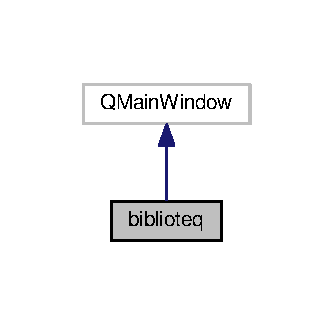
\includegraphics[width=160pt]{classbiblioteq__inherit__graph}
\end{center}
\end{figure}


Collaboration diagram for biblioteq\+:
\nopagebreak
\begin{figure}[H]
\begin{center}
\leavevmode
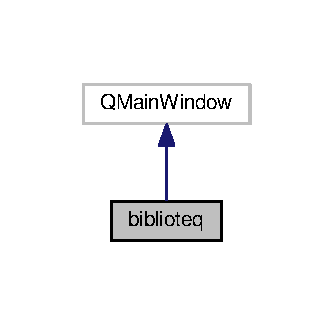
\includegraphics[width=160pt]{classbiblioteq__coll__graph}
\end{center}
\end{figure}
\subsection*{Public Slots}
\begin{DoxyCompactItemize}
\item 
void {\bfseries slot\+Display\+Summary} (void)\hypertarget{classbiblioteq_a857a2b520a0011809ab4ba9f6684ae6e}{}\label{classbiblioteq_a857a2b520a0011809ab4ba9f6684ae6e}

\item 
void {\bfseries slot\+Resize\+Columns} (void)\hypertarget{classbiblioteq_a2b5613a73c87cbd2efb1b63701c5a453}{}\label{classbiblioteq_a2b5613a73c87cbd2efb1b63701c5a453}

\end{DoxyCompactItemize}
\subsection*{Public Member Functions}
\begin{DoxyCompactItemize}
\item 
Q\+Hash$<$ Q\+String, Q\+String $>$ {\bfseries get\+Amazon\+Hash} (void) const \hypertarget{classbiblioteq_a3618108d9eed5862cec1ee7194cb27bf}{}\label{classbiblioteq_a3618108d9eed5862cec1ee7194cb27bf}

\item 
Q\+Main\+Window $\ast$ {\bfseries get\+Members\+Browser} (void) const \hypertarget{classbiblioteq_ab8260306aa44418a9b109fc26270f176}{}\label{classbiblioteq_ab8260306aa44418a9b109fc26270f176}

\item 
Q\+Map$<$ Q\+String, Q\+Hash$<$ Q\+String, Q\+String $>$ $>$ {\bfseries get\+S\+R\+U\+Maps} (void) const \hypertarget{classbiblioteq_ab46fd3374287959c3f13216ec5fdc179}{}\label{classbiblioteq_ab46fd3374287959c3f13216ec5fdc179}

\item 
Q\+Map$<$ Q\+String, Q\+Hash$<$ Q\+String, Q\+String $>$ $>$ {\bfseries get\+Z3950\+Maps} (void) const \hypertarget{classbiblioteq_af47999e074de54cec2af68b040042ef2}{}\label{classbiblioteq_af47999e074de54cec2af68b040042ef2}

\item 
Q\+Sql\+Database {\bfseries get\+DB} (void) const \hypertarget{classbiblioteq_af6782af753826b7239b9e379490baa70}{}\label{classbiblioteq_af6782af753826b7239b9e379490baa70}

\item 
Q\+String {\bfseries get\+Admin\+ID} (void) const \hypertarget{classbiblioteq_a64256300b17c43e1889f2ec022226b39}{}\label{classbiblioteq_a64256300b17c43e1889f2ec022226b39}

\item 
Q\+String {\bfseries get\+Preferred\+S\+R\+U\+Site} (void) const \hypertarget{classbiblioteq_a7c9e5e9dc065598804fefc5e5c6e5492}{}\label{classbiblioteq_a7c9e5e9dc065598804fefc5e5c6e5492}

\item 
Q\+String {\bfseries get\+Preferred\+Z3950\+Site} (void) const \hypertarget{classbiblioteq_a4c4625515fa8dbdb3d26a39af919c25d}{}\label{classbiblioteq_a4c4625515fa8dbdb3d26a39af919c25d}

\item 
Q\+String {\bfseries get\+Roles} (void) const \hypertarget{classbiblioteq_a65c95e919984ca1d0c6c7f74ad95310f}{}\label{classbiblioteq_a65c95e919984ca1d0c6c7f74ad95310f}

\item 
Q\+String {\bfseries get\+Type\+Filter\+String} (void) const \hypertarget{classbiblioteq_a8c232e081602550c2eaa584d7d532f64}{}\label{classbiblioteq_a8c232e081602550c2eaa584d7d532f64}

\item 
Q\+String {\bfseries publication\+Date\+Format} (const Q\+String \&item\+Type) const \hypertarget{classbiblioteq_a1ce8f17d9436b9d049dd3e4a39ec5ecd}{}\label{classbiblioteq_a1ce8f17d9436b9d049dd3e4a39ec5ecd}

\item 
Q\+Variant {\bfseries setting} (const Q\+String \&name) const \hypertarget{classbiblioteq_a329db5ca10eda04fad3fe09ce6d36bad}{}\label{classbiblioteq_a329db5ca10eda04fad3fe09ce6d36bad}

\item 
Q\+Vector$<$ Q\+String $>$ {\bfseries get\+B\+B\+Column\+Indexes} (void) const \hypertarget{classbiblioteq_a78abafa3af180949743cfe885eade850}{}\label{classbiblioteq_a78abafa3af180949743cfe885eade850}

\item 
Ui\+\_\+main\+Window {\bfseries get\+UI} (void) const \hypertarget{classbiblioteq_adec28d45f9ddc0060cc60a9f561a477f}{}\label{classbiblioteq_adec28d45f9ddc0060cc60a9f561a477f}

\item 
Ui\+\_\+members\+Browser {\bfseries get\+BB} (void) const \hypertarget{classbiblioteq_a5097015273e31dfd3946440d13cc69d8}{}\label{classbiblioteq_a5097015273e31dfd3946440d13cc69d8}

\item 
bool {\bfseries is\+Guest} (void) const \hypertarget{classbiblioteq_a321d120a6ff753f3e5240fe40e1e746f}{}\label{classbiblioteq_a321d120a6ff753f3e5240fe40e1e746f}

\item 
int {\bfseries populate\+Table} (const int search\+\_\+type\+\_\+arg, const Q\+String \&typefilter, const Q\+String \&searchstr\+Arg, const int paging\+Type=N\+E\+W\+\_\+\+P\+A\+GE)\hypertarget{classbiblioteq_ae13409ea2011c0dde922530b1fbba8d0}{}\label{classbiblioteq_ae13409ea2011c0dde922530b1fbba8d0}

\item 
void {\bfseries add\+Error} (const Q\+String \&type, const Q\+String \&summary, const Q\+String \&error=\char`\"{}\char`\"{}, const char $\ast$file=\char`\"{}\char`\"{}, const int line=0)\hypertarget{classbiblioteq_a6773c729ae670a40b804ad9a5609ffb2}{}\label{classbiblioteq_a6773c729ae670a40b804ad9a5609ffb2}

\item 
void {\bfseries book\+Search} (const Q\+String \&field, const Q\+String \&value)\hypertarget{classbiblioteq_a42c5a134c4e911e157fd1b6e694c5452}{}\label{classbiblioteq_a42c5a134c4e911e157fd1b6e694c5452}

\item 
void {\bfseries cd\+Search} (const Q\+String \&field, const Q\+String \&value)\hypertarget{classbiblioteq_a3ea36c2342bc706c3b7fbbc61c720de0}{}\label{classbiblioteq_a3ea36c2342bc706c3b7fbbc61c720de0}

\item 
void {\bfseries dvd\+Search} (const Q\+String \&field, const Q\+String \&value)\hypertarget{classbiblioteq_a33ba3747af1b89b420dc813cda8d8842}{}\label{classbiblioteq_a33ba3747af1b89b420dc813cda8d8842}

\item 
void {\bfseries journ\+Search} (const Q\+String \&field, const Q\+String \&value)\hypertarget{classbiblioteq_a498e7e1e73f177af81c844626e4c5ee1}{}\label{classbiblioteq_a498e7e1e73f177af81c844626e4c5ee1}

\item 
void {\bfseries mag\+Search} (const Q\+String \&field, const Q\+String \&value)\hypertarget{classbiblioteq_a015f420e14b8b277de870d317275289d}{}\label{classbiblioteq_a015f420e14b8b277de870d317275289d}

\item 
void {\bfseries pc\+Search} (const Q\+String \&field, const Q\+String \&value)\hypertarget{classbiblioteq_a2c0e14a67b18f830933fd457b6d6bc5a}{}\label{classbiblioteq_a2c0e14a67b18f830933fd457b6d6bc5a}

\item 
void {\bfseries remove\+Book} (\hyperlink{classbiblioteq__book}{biblioteq\+\_\+book} $\ast$book)\hypertarget{classbiblioteq_a2979cfdcec7595bddc0f2d0447803260}{}\label{classbiblioteq_a2979cfdcec7595bddc0f2d0447803260}

\item 
void {\bfseries remove\+CD} (\hyperlink{classbiblioteq__cd}{biblioteq\+\_\+cd} $\ast$cd)\hypertarget{classbiblioteq_ab00724d6107603490dd5ecccdfd66704}{}\label{classbiblioteq_ab00724d6107603490dd5ecccdfd66704}

\item 
void {\bfseries remove\+D\+VD} (\hyperlink{classbiblioteq__dvd}{biblioteq\+\_\+dvd} $\ast$dvd)\hypertarget{classbiblioteq_a4e50365e71f53b9d89c3fe929dc30566}{}\label{classbiblioteq_a4e50365e71f53b9d89c3fe929dc30566}

\item 
void {\bfseries remove\+Journal} (\hyperlink{classbiblioteq__journal}{biblioteq\+\_\+journal} $\ast$journal)\hypertarget{classbiblioteq_a0f0ef4b0727fc0b382f7e0efd05eb56c}{}\label{classbiblioteq_a0f0ef4b0727fc0b382f7e0efd05eb56c}

\item 
void {\bfseries remove\+Magazine} (\hyperlink{classbiblioteq__magazine}{biblioteq\+\_\+magazine} $\ast$magazine)\hypertarget{classbiblioteq_a7c37e0b965155c55477dc77ffdc44d0c}{}\label{classbiblioteq_a7c37e0b965155c55477dc77ffdc44d0c}

\item 
void {\bfseries remove\+Photograph\+Collection} (\hyperlink{classbiblioteq__photographcollection}{biblioteq\+\_\+photographcollection} $\ast$pc)\hypertarget{classbiblioteq_a5e581fcca72d629a4b2c0d1bf7f86faa}{}\label{classbiblioteq_a5e581fcca72d629a4b2c0d1bf7f86faa}

\item 
void {\bfseries remove\+Video\+Game} (\hyperlink{classbiblioteq__videogame}{biblioteq\+\_\+videogame} $\ast$videogame)\hypertarget{classbiblioteq_a1d6c81d17b07a84ae48474c7a00d0ba8}{}\label{classbiblioteq_a1d6c81d17b07a84ae48474c7a00d0ba8}

\item 
void {\bfseries replace\+Book} (const Q\+String \&id, \hyperlink{classbiblioteq__book}{biblioteq\+\_\+book} $\ast$book)\hypertarget{classbiblioteq_a30d09d4fa9241f0566ca5378f8031db1}{}\label{classbiblioteq_a30d09d4fa9241f0566ca5378f8031db1}

\item 
void {\bfseries replace\+CD} (const Q\+String \&id, \hyperlink{classbiblioteq__cd}{biblioteq\+\_\+cd} $\ast$cd)\hypertarget{classbiblioteq_a158fb9bccec884e7ac11a624017735bd}{}\label{classbiblioteq_a158fb9bccec884e7ac11a624017735bd}

\item 
void {\bfseries replace\+D\+VD} (const Q\+String \&id, \hyperlink{classbiblioteq__dvd}{biblioteq\+\_\+dvd} $\ast$dvd)\hypertarget{classbiblioteq_aee527720c5b3e27aa8bce2285ba5c9ff}{}\label{classbiblioteq_aee527720c5b3e27aa8bce2285ba5c9ff}

\item 
void {\bfseries replace\+Journal} (const Q\+String \&id, \hyperlink{classbiblioteq__journal}{biblioteq\+\_\+journal} $\ast$journal)\hypertarget{classbiblioteq_adcfba86f54a0cff1e51961ff56c0feb8}{}\label{classbiblioteq_adcfba86f54a0cff1e51961ff56c0feb8}

\item 
void {\bfseries replace\+Magazine} (const Q\+String \&id, \hyperlink{classbiblioteq__magazine}{biblioteq\+\_\+magazine} $\ast$magazine)\hypertarget{classbiblioteq_a72beeff6b5eee53f977a686258c0b10f}{}\label{classbiblioteq_a72beeff6b5eee53f977a686258c0b10f}

\item 
void {\bfseries replace\+Photograph\+Collection} (const Q\+String \&id, \hyperlink{classbiblioteq__photographcollection}{biblioteq\+\_\+photographcollection} $\ast$pc)\hypertarget{classbiblioteq_a87358d5db660dec1c31d39a4142eee02}{}\label{classbiblioteq_a87358d5db660dec1c31d39a4142eee02}

\item 
void {\bfseries replace\+Video\+Game} (const Q\+String \&id, \hyperlink{classbiblioteq__videogame}{biblioteq\+\_\+videogame} $\ast$videogame)\hypertarget{classbiblioteq_a1fa674db3d30a09869c462d64d218164}{}\label{classbiblioteq_a1fa674db3d30a09869c462d64d218164}

\item 
void {\bfseries set\+Global\+Fonts} (const Q\+Font \&font)\hypertarget{classbiblioteq_a40009f0c4c0e42a784749d41a9e0c7ba}{}\label{classbiblioteq_a40009f0c4c0e42a784749d41a9e0c7ba}

\item 
void {\bfseries show\+Main} (void)\hypertarget{classbiblioteq_a4b14ed8e19b0f98c22a4dafde90a8baa}{}\label{classbiblioteq_a4b14ed8e19b0f98c22a4dafde90a8baa}

\item 
void {\bfseries update\+Item\+Windows} (void)\hypertarget{classbiblioteq_a8e5d924b22bd5bbff09605e2c4274e6f}{}\label{classbiblioteq_a8e5d924b22bd5bbff09605e2c4274e6f}

\item 
void {\bfseries update\+Members\+Browser} (const Q\+String \&memberid)\hypertarget{classbiblioteq_ae0b6755aa5ec54fe2cb5bb6842f95a55}{}\label{classbiblioteq_ae0b6755aa5ec54fe2cb5bb6842f95a55}

\item 
void {\bfseries update\+Members\+Browser} (void)\hypertarget{classbiblioteq_af25cd59010d3b98dc840d399602a24d5}{}\label{classbiblioteq_af25cd59010d3b98dc840d399602a24d5}

\item 
void {\bfseries update\+Reservation\+History\+Browser} (const Q\+String \&memberid, const Q\+String \&ioid, const Q\+String \&copyid, const Q\+String \&item\+Type, const Q\+String \&returned\+Date)\hypertarget{classbiblioteq_adc5582f65430cb8e7c4fde7c61c6ceb6}{}\label{classbiblioteq_adc5582f65430cb8e7c4fde7c61c6ceb6}

\item 
void {\bfseries update\+Rows} (const Q\+String \&oid, const int row, const Q\+String \&item\+Type)\hypertarget{classbiblioteq_a486b9abc9d7c0d682c1d991c1cf81496}{}\label{classbiblioteq_a486b9abc9d7c0d682c1d991c1cf81496}

\item 
void {\bfseries update\+Scene\+Item} (const Q\+String \&oid, const Q\+String \&type, const Q\+Image \&image)\hypertarget{classbiblioteq_aa95f6bd6c1294be28f09d7e7454aa35b}{}\label{classbiblioteq_aa95f6bd6c1294be28f09d7e7454aa35b}

\item 
void {\bfseries vg\+Search} (const Q\+String \&field, const Q\+String \&value)\hypertarget{classbiblioteq_a9b3730fd94a7ff095b983f25b0934ca9}{}\label{classbiblioteq_a9b3730fd94a7ff095b983f25b0934ca9}

\end{DoxyCompactItemize}
\subsection*{Static Public Member Functions}
\begin{DoxyCompactItemize}
\item 
static Q\+String {\bfseries home\+Path} (void)\hypertarget{classbiblioteq_a77dff33726661558d8d93b8b681d8650}{}\label{classbiblioteq_a77dff33726661558d8d93b8b681d8650}

\item 
static void {\bfseries quit} (const char $\ast$msg, const char $\ast$file, const int line)\hypertarget{classbiblioteq_aaddc108d0fe310ea1af60fed14bc80f3}{}\label{classbiblioteq_aaddc108d0fe310ea1af60fed14bc80f3}

\item 
static void {\bfseries quit} (void)\hypertarget{classbiblioteq_a3ffe0cfcba2b0bda0cd13e79047d25d6}{}\label{classbiblioteq_a3ffe0cfcba2b0bda0cd13e79047d25d6}

\end{DoxyCompactItemize}
\subsection*{Public Attributes}
\begin{DoxyCompactItemize}
\item 
Q\+Menu $\ast$ {\bfseries m\+\_\+config\+Tool\+Menu}\hypertarget{classbiblioteq_a221649d43f277d9ab329144b2af8dca9}{}\label{classbiblioteq_a221649d43f277d9ab329144b2af8dca9}

\end{DoxyCompactItemize}
\subsection*{Static Public Attributes}
\begin{DoxyCompactItemize}
\item 
static Q\+String {\bfseries s\+\_\+locale} = \char`\"{}\char`\"{}\hypertarget{classbiblioteq_a531cce7604bd675011719b1ca767081f}{}\label{classbiblioteq_a531cce7604bd675011719b1ca767081f}

\item 
static Q\+Translator $\ast$ {\bfseries s\+\_\+app\+Translator} = 0\hypertarget{classbiblioteq_ab62168fc59cdc975ed118587acc643f4}{}\label{classbiblioteq_ab62168fc59cdc975ed118587acc643f4}

\item 
static Q\+Translator $\ast$ {\bfseries s\+\_\+qt\+Translator} = 0\hypertarget{classbiblioteq_a63e565603b391d30909c382e9a648a20}{}\label{classbiblioteq_a63e565603b391d30909c382e9a648a20}

\item 
static const int {\bfseries C\+U\+S\+T\+O\+M\+\_\+\+Q\+U\+E\+RY} = 0\hypertarget{classbiblioteq_ad32b3a87e24c6da29ad38e82a5621a74}{}\label{classbiblioteq_ad32b3a87e24c6da29ad38e82a5621a74}

\item 
static const int {\bfseries E\+D\+I\+T\+A\+B\+LE} = 0\hypertarget{classbiblioteq_a6428b315b0e99be77392694e701e6613}{}\label{classbiblioteq_a6428b315b0e99be77392694e701e6613}

\item 
static const int {\bfseries N\+E\+W\+\_\+\+P\+A\+GE} = 0\hypertarget{classbiblioteq_a6d7869e8f55f035a4579dbfbdcc7ae90}{}\label{classbiblioteq_a6d7869e8f55f035a4579dbfbdcc7ae90}

\item 
static const int {\bfseries N\+E\+X\+T\+\_\+\+P\+A\+GE} = 1\hypertarget{classbiblioteq_a4e6e213d931046a9ae10fcfb89cd4080}{}\label{classbiblioteq_a4e6e213d931046a9ae10fcfb89cd4080}

\item 
static const int {\bfseries P\+O\+P\+U\+L\+A\+T\+E\+\_\+\+A\+LL} = 1\hypertarget{classbiblioteq_a60719fb6ee0ebb342d9cc10771503d3f}{}\label{classbiblioteq_a60719fb6ee0ebb342d9cc10771503d3f}

\item 
static const int {\bfseries P\+O\+P\+U\+L\+A\+T\+E\+\_\+\+S\+E\+A\+R\+CH} = 2\hypertarget{classbiblioteq_a09b1c95cd2e1949a5d2d8b2c13c76042}{}\label{classbiblioteq_a09b1c95cd2e1949a5d2d8b2c13c76042}

\item 
static const int {\bfseries P\+O\+P\+U\+L\+A\+T\+E\+\_\+\+S\+E\+A\+R\+C\+H\+\_\+\+B\+A\+S\+IC} = 3\hypertarget{classbiblioteq_a6a528227ec1b55674079308da819ca21}{}\label{classbiblioteq_a6a528227ec1b55674079308da819ca21}

\item 
static const int {\bfseries P\+R\+E\+V\+I\+O\+U\+S\+\_\+\+P\+A\+GE} = 2\hypertarget{classbiblioteq_a68406e00aad96ddd05dd6ff2d9017f5f}{}\label{classbiblioteq_a68406e00aad96ddd05dd6ff2d9017f5f}

\item 
static const int {\bfseries V\+I\+E\+W\+\_\+\+O\+N\+LY} = 1\hypertarget{classbiblioteq_a11f44b308723c9036be111822a8307be}{}\label{classbiblioteq_a11f44b308723c9036be111822a8307be}

\end{DoxyCompactItemize}


The documentation for this class was generated from the following files\+:\begin{DoxyCompactItemize}
\item 
Source/biblioteq.\+h\item 
Source/biblioteq\+\_\+a.\+cc\item 
Source/biblioteq\+\_\+b.\+cc\item 
Source/biblioteq\+\_\+c.\+cc\end{DoxyCompactItemize}

\hypertarget{classbiblioteq__bgraphicsscene}{}\section{biblioteq\+\_\+bgraphicsscene Class Reference}
\label{classbiblioteq__bgraphicsscene}\index{biblioteq\+\_\+bgraphicsscene@{biblioteq\+\_\+bgraphicsscene}}


Inheritance diagram for biblioteq\+\_\+bgraphicsscene\+:
\nopagebreak
\begin{figure}[H]
\begin{center}
\leavevmode
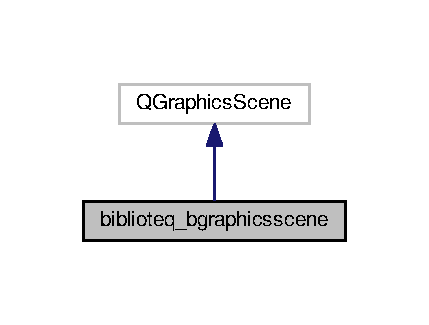
\includegraphics[width=206pt]{classbiblioteq__bgraphicsscene__inherit__graph}
\end{center}
\end{figure}


Collaboration diagram for biblioteq\+\_\+bgraphicsscene\+:
\nopagebreak
\begin{figure}[H]
\begin{center}
\leavevmode
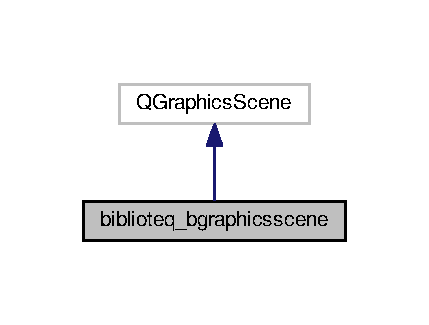
\includegraphics[width=206pt]{classbiblioteq__bgraphicsscene__coll__graph}
\end{center}
\end{figure}
\subsection*{Signals}
\begin{DoxyCompactItemize}
\item 
void {\bfseries delete\+Key\+Pressed} (void)\hypertarget{classbiblioteq__bgraphicsscene_a8553f29440d58e306eba748ed0d96135}{}\label{classbiblioteq__bgraphicsscene_a8553f29440d58e306eba748ed0d96135}

\item 
void {\bfseries item\+Double\+Clicked} (void)\hypertarget{classbiblioteq__bgraphicsscene_affd52d53ab37e9ff7a3aaeeda1713b23}{}\label{classbiblioteq__bgraphicsscene_affd52d53ab37e9ff7a3aaeeda1713b23}

\end{DoxyCompactItemize}
\subsection*{Public Member Functions}
\begin{DoxyCompactItemize}
\item 
{\bfseries biblioteq\+\_\+bgraphicsscene} (Q\+Object $\ast$parent)\hypertarget{classbiblioteq__bgraphicsscene_a7f6d955afd7852faccb4b7c5e2f1afd2}{}\label{classbiblioteq__bgraphicsscene_a7f6d955afd7852faccb4b7c5e2f1afd2}

\end{DoxyCompactItemize}


The documentation for this class was generated from the following files\+:\begin{DoxyCompactItemize}
\item 
Source/biblioteq\+\_\+bgraphicsscene.\+h\item 
Source/biblioteq\+\_\+bgraphicsscene.\+cc\end{DoxyCompactItemize}

\hypertarget{classbiblioteq__book}{}\section{biblioteq\+\_\+book Class Reference}
\label{classbiblioteq__book}\index{biblioteq\+\_\+book@{biblioteq\+\_\+book}}


Inheritance diagram for biblioteq\+\_\+book\+:
\nopagebreak
\begin{figure}[H]
\begin{center}
\leavevmode
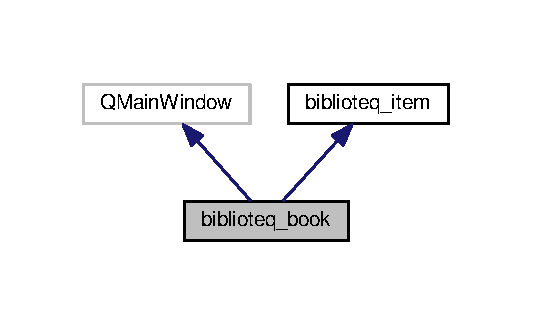
\includegraphics[width=256pt]{classbiblioteq__book__inherit__graph}
\end{center}
\end{figure}


Collaboration diagram for biblioteq\+\_\+book\+:
\nopagebreak
\begin{figure}[H]
\begin{center}
\leavevmode
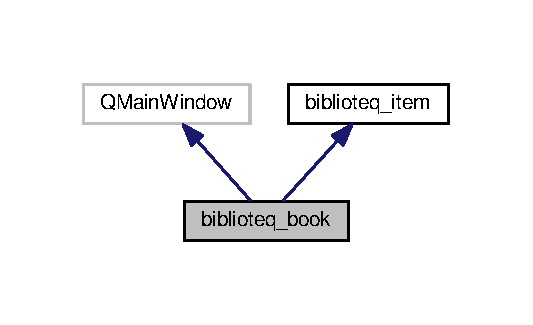
\includegraphics[width=256pt]{classbiblioteq__book__coll__graph}
\end{center}
\end{figure}
\subsection*{Public Member Functions}
\begin{DoxyCompactItemize}
\item 
{\bfseries biblioteq\+\_\+book} (Q\+Main\+Window $\ast$parent\+Arg, const Q\+String \&oid\+Arg, const int row\+Arg)\hypertarget{classbiblioteq__book_a9c49be1b86b1271b29c62ac080c7d690}{}\label{classbiblioteq__book_a9c49be1b86b1271b29c62ac080c7d690}

\item 
void {\bfseries duplicate} (const Q\+String \&p\+\_\+oid, const int state)\hypertarget{classbiblioteq__book_a94e9438ea4efeb2b09655868528a0e66}{}\label{classbiblioteq__book_a94e9438ea4efeb2b09655868528a0e66}

\item 
void {\bfseries insert} (void)\hypertarget{classbiblioteq__book_af6bc97dae293a25690f436c3c3909b8d}{}\label{classbiblioteq__book_af6bc97dae293a25690f436c3c3909b8d}

\item 
void {\bfseries modify} (const int state)\hypertarget{classbiblioteq__book_a89e33d0067a5970384d3ae2215f4e691}{}\label{classbiblioteq__book_a89e33d0067a5970384d3ae2215f4e691}

\item 
void {\bfseries search} (const Q\+String \&field=\char`\"{}\char`\"{}, const Q\+String \&value=\char`\"{}\char`\"{})\hypertarget{classbiblioteq__book_a9fc5c29f9a288cc220708843f454cb3b}{}\label{classbiblioteq__book_a9fc5c29f9a288cc220708843f454cb3b}

\item 
void {\bfseries set\+Publication\+Date\+Format} (const Q\+String \&date\+Format)\hypertarget{classbiblioteq__book_a0fe820b8616f9cb6b441f47d7189aeed}{}\label{classbiblioteq__book_a0fe820b8616f9cb6b441f47d7189aeed}

\item 
void {\bfseries update\+Window} (const int)\hypertarget{classbiblioteq__book_a472b0af8e34398364f759b1af9c6b239}{}\label{classbiblioteq__book_a472b0af8e34398364f759b1af9c6b239}

\end{DoxyCompactItemize}
\subsection*{Additional Inherited Members}


The documentation for this class was generated from the following files\+:\begin{DoxyCompactItemize}
\item 
Source/biblioteq\+\_\+book.\+h\item 
Source/biblioteq\+\_\+book.\+cc\end{DoxyCompactItemize}

\hypertarget{classbiblioteq__borrowers__editor}{}\section{biblioteq\+\_\+borrowers\+\_\+editor Class Reference}
\label{classbiblioteq__borrowers__editor}\index{biblioteq\+\_\+borrowers\+\_\+editor@{biblioteq\+\_\+borrowers\+\_\+editor}}


Inheritance diagram for biblioteq\+\_\+borrowers\+\_\+editor\+:
\nopagebreak
\begin{figure}[H]
\begin{center}
\leavevmode
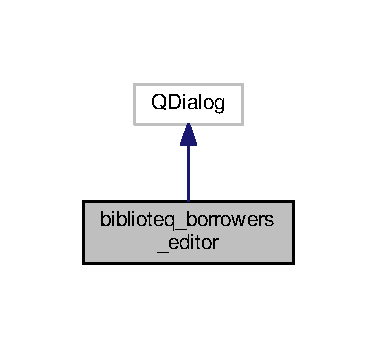
\includegraphics[width=181pt]{classbiblioteq__borrowers__editor__inherit__graph}
\end{center}
\end{figure}


Collaboration diagram for biblioteq\+\_\+borrowers\+\_\+editor\+:
\nopagebreak
\begin{figure}[H]
\begin{center}
\leavevmode
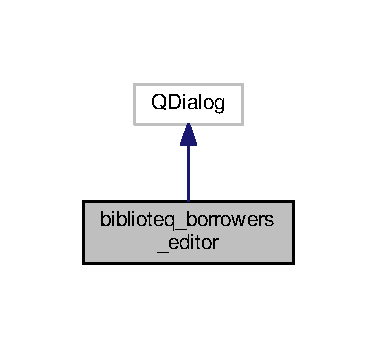
\includegraphics[width=181pt]{classbiblioteq__borrowers__editor__coll__graph}
\end{center}
\end{figure}
\subsection*{Public Member Functions}
\begin{DoxyCompactItemize}
\item 
{\bfseries biblioteq\+\_\+borrowers\+\_\+editor} (Q\+Widget $\ast$parent, \hyperlink{classbiblioteq__item}{biblioteq\+\_\+item} $\ast$bitem\+Arg, const int quantity\+Arg, const Q\+String \&ioid\+Arg, const Q\+String \&uniqueid\+Arg, const Q\+Font \&font, const Q\+String \&item\+Type\+Arg, const int state\+Arg)\hypertarget{classbiblioteq__borrowers__editor_a1215ea5da84e858cb1438c537f32d7da}{}\label{classbiblioteq__borrowers__editor_a1215ea5da84e858cb1438c537f32d7da}

\item 
void {\bfseries show\+Users} (void)\hypertarget{classbiblioteq__borrowers__editor_a300cf57e5ddbe8734f1c8e8ff05a5f1a}{}\label{classbiblioteq__borrowers__editor_a300cf57e5ddbe8734f1c8e8ff05a5f1a}

\end{DoxyCompactItemize}


The documentation for this class was generated from the following files\+:\begin{DoxyCompactItemize}
\item 
Source/biblioteq\+\_\+borrowers\+\_\+editor.\+h\item 
Source/biblioteq\+\_\+borrowers\+\_\+editor.\+cc\end{DoxyCompactItemize}

\hypertarget{classbiblioteq__callnum__table__item}{}\section{biblioteq\+\_\+callnum\+\_\+table\+\_\+item Class Reference}
\label{classbiblioteq__callnum__table__item}\index{biblioteq\+\_\+callnum\+\_\+table\+\_\+item@{biblioteq\+\_\+callnum\+\_\+table\+\_\+item}}


Inheritance diagram for biblioteq\+\_\+callnum\+\_\+table\+\_\+item\+:
\nopagebreak
\begin{figure}[H]
\begin{center}
\leavevmode
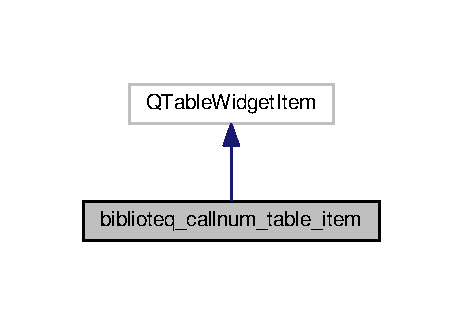
\includegraphics[width=222pt]{classbiblioteq__callnum__table__item__inherit__graph}
\end{center}
\end{figure}


Collaboration diagram for biblioteq\+\_\+callnum\+\_\+table\+\_\+item\+:
\nopagebreak
\begin{figure}[H]
\begin{center}
\leavevmode
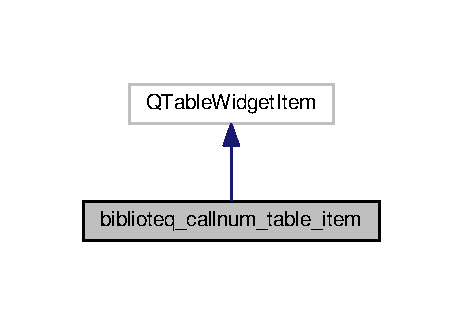
\includegraphics[width=222pt]{classbiblioteq__callnum__table__item__coll__graph}
\end{center}
\end{figure}
\subsection*{Public Member Functions}
\begin{DoxyCompactItemize}
\item 
{\bfseries biblioteq\+\_\+callnum\+\_\+table\+\_\+item} (const Q\+String \&str)\hypertarget{classbiblioteq__callnum__table__item_aefca59d2ee38775e9f03c3bfb1b9128d}{}\label{classbiblioteq__callnum__table__item_aefca59d2ee38775e9f03c3bfb1b9128d}

\item 
bool {\bfseries operator$<$} (const Q\+Table\+Widget\+Item \&other) const \hypertarget{classbiblioteq__callnum__table__item_a45f885106fa28e607ac09e8503ccd987}{}\label{classbiblioteq__callnum__table__item_a45f885106fa28e607ac09e8503ccd987}

\end{DoxyCompactItemize}


The documentation for this class was generated from the following files\+:\begin{DoxyCompactItemize}
\item 
Source/biblioteq\+\_\+callnum\+\_\+table\+\_\+item.\+h\item 
Source/biblioteq\+\_\+callnum\+\_\+table\+\_\+item.\+cc\end{DoxyCompactItemize}

\hypertarget{classbiblioteq__cd}{}\section{biblioteq\+\_\+cd Class Reference}
\label{classbiblioteq__cd}\index{biblioteq\+\_\+cd@{biblioteq\+\_\+cd}}


Inheritance diagram for biblioteq\+\_\+cd\+:
\nopagebreak
\begin{figure}[H]
\begin{center}
\leavevmode
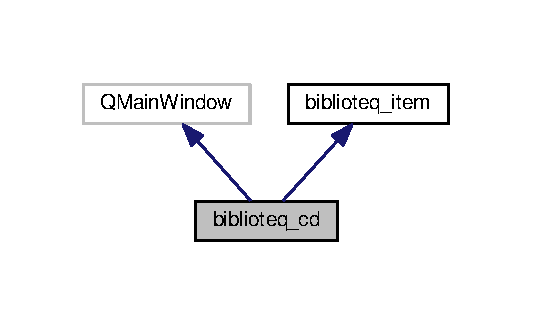
\includegraphics[width=256pt]{classbiblioteq__cd__inherit__graph}
\end{center}
\end{figure}


Collaboration diagram for biblioteq\+\_\+cd\+:
\nopagebreak
\begin{figure}[H]
\begin{center}
\leavevmode
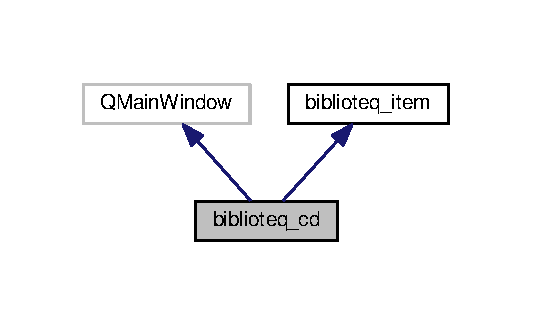
\includegraphics[width=256pt]{classbiblioteq__cd__coll__graph}
\end{center}
\end{figure}
\subsection*{Public Member Functions}
\begin{DoxyCompactItemize}
\item 
{\bfseries biblioteq\+\_\+cd} (Q\+Main\+Window $\ast$parent\+Arg, const Q\+String \&oid\+Arg, const int row\+Arg)\hypertarget{classbiblioteq__cd_a060f54400243040c2374960a4f27bf40}{}\label{classbiblioteq__cd_a060f54400243040c2374960a4f27bf40}

\item 
void {\bfseries duplicate} (const Q\+String \&p\+\_\+oid, const int state)\hypertarget{classbiblioteq__cd_ae240accaf0c6d7d07effc54402b45f40}{}\label{classbiblioteq__cd_ae240accaf0c6d7d07effc54402b45f40}

\item 
void {\bfseries insert} (void)\hypertarget{classbiblioteq__cd_a29cb088f999555ed2d63b323b717b68f}{}\label{classbiblioteq__cd_a29cb088f999555ed2d63b323b717b68f}

\item 
void {\bfseries modify} (const int state)\hypertarget{classbiblioteq__cd_a0e2a26b8108bee92eb780a218fab7e7c}{}\label{classbiblioteq__cd_a0e2a26b8108bee92eb780a218fab7e7c}

\item 
void {\bfseries search} (const Q\+String \&field=\char`\"{}\char`\"{}, const Q\+String \&value=\char`\"{}\char`\"{})\hypertarget{classbiblioteq__cd_a0071b1a6d28b89c29b6ef94a9c701ae9}{}\label{classbiblioteq__cd_a0071b1a6d28b89c29b6ef94a9c701ae9}

\item 
void {\bfseries set\+Publication\+Date\+Format} (const Q\+String \&date\+Format)\hypertarget{classbiblioteq__cd_a080477c718d7c3fe6fdafc6915484df1}{}\label{classbiblioteq__cd_a080477c718d7c3fe6fdafc6915484df1}

\item 
void {\bfseries update\+Window} (const int)\hypertarget{classbiblioteq__cd_ae42d2fc452a5d3aebdfb162bf655cc3b}{}\label{classbiblioteq__cd_ae42d2fc452a5d3aebdfb162bf655cc3b}

\end{DoxyCompactItemize}
\subsection*{Additional Inherited Members}


The documentation for this class was generated from the following files\+:\begin{DoxyCompactItemize}
\item 
Source/biblioteq\+\_\+cd.\+h\item 
Source/biblioteq\+\_\+cd.\+cc\end{DoxyCompactItemize}

\hypertarget{classbiblioteq__copy__editor}{}\section{biblioteq\+\_\+copy\+\_\+editor Class Reference}
\label{classbiblioteq__copy__editor}\index{biblioteq\+\_\+copy\+\_\+editor@{biblioteq\+\_\+copy\+\_\+editor}}


Inheritance diagram for biblioteq\+\_\+copy\+\_\+editor\+:
\nopagebreak
\begin{figure}[H]
\begin{center}
\leavevmode
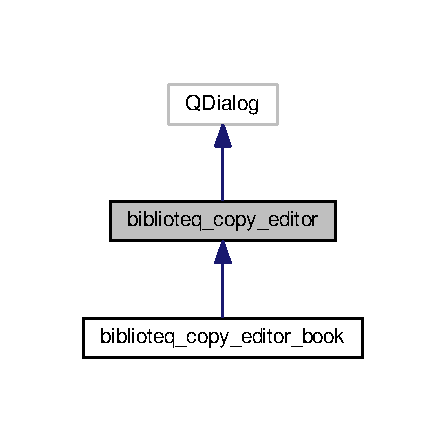
\includegraphics[width=214pt]{classbiblioteq__copy__editor__inherit__graph}
\end{center}
\end{figure}


Collaboration diagram for biblioteq\+\_\+copy\+\_\+editor\+:
\nopagebreak
\begin{figure}[H]
\begin{center}
\leavevmode
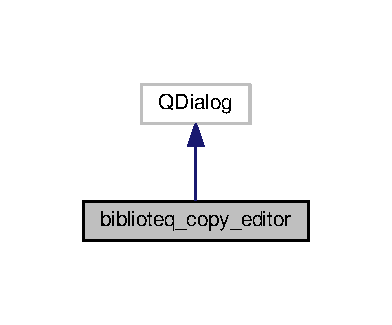
\includegraphics[width=188pt]{classbiblioteq__copy__editor__coll__graph}
\end{center}
\end{figure}
\subsection*{Public Member Functions}
\begin{DoxyCompactItemize}
\item 
{\bfseries biblioteq\+\_\+copy\+\_\+editor} (Q\+Widget $\ast$parent)\hypertarget{classbiblioteq__copy__editor_a6cceb037e03461cb0d4e5a0d3d489816}{}\label{classbiblioteq__copy__editor_a6cceb037e03461cb0d4e5a0d3d489816}

\item 
{\bfseries biblioteq\+\_\+copy\+\_\+editor} (Q\+Widget $\ast$parent, \hyperlink{classbiblioteq__item}{biblioteq\+\_\+item} $\ast$bitem\+Arg, const bool show\+For\+Lending\+Arg, const int quantity\+Arg, const Q\+String \&ioid\+Arg, Q\+Spin\+Box $\ast$spinbox\+Arg, const Q\+Font \&font, const Q\+String \&item\+Type\+Arg, const Q\+String \&unique\+Id\+Arg)\hypertarget{classbiblioteq__copy__editor_ac0b0f73f588a1722dc8246bf47605f00}{}\label{classbiblioteq__copy__editor_ac0b0f73f588a1722dc8246bf47605f00}

\item 
void {\bfseries populate\+Copies\+Editor} (void)\hypertarget{classbiblioteq__copy__editor_aef96ac95e48bfed49407d25437aaf493}{}\label{classbiblioteq__copy__editor_aef96ac95e48bfed49407d25437aaf493}

\end{DoxyCompactItemize}
\subsection*{Protected Slots}
\begin{DoxyCompactItemize}
\item 
void {\bfseries slot\+Close\+Copy\+Editor} (void)\hypertarget{classbiblioteq__copy__editor_a2b8e609c6700813a918e19c0171d3e40}{}\label{classbiblioteq__copy__editor_a2b8e609c6700813a918e19c0171d3e40}

\end{DoxyCompactItemize}
\subsection*{Protected Member Functions}
\begin{DoxyCompactItemize}
\item 
void {\bfseries clear\+Copies\+List} (void)\hypertarget{classbiblioteq__copy__editor_a7ac49564b84dd0f3095c5ab4ddc4fe63}{}\label{classbiblioteq__copy__editor_a7ac49564b84dd0f3095c5ab4ddc4fe63}

\item 
void {\bfseries set\+Global\+Fonts} (const Q\+Font \&font)\hypertarget{classbiblioteq__copy__editor_aea18dad7328884d26c2e7d03770aa14b}{}\label{classbiblioteq__copy__editor_aea18dad7328884d26c2e7d03770aa14b}

\end{DoxyCompactItemize}


The documentation for this class was generated from the following files\+:\begin{DoxyCompactItemize}
\item 
Source/biblioteq\+\_\+copy\+\_\+editor.\+h\item 
Source/biblioteq\+\_\+copy\+\_\+editor.\+cc\end{DoxyCompactItemize}

\hypertarget{classbiblioteq__copy__editor__book}{}\section{biblioteq\+\_\+copy\+\_\+editor\+\_\+book Class Reference}
\label{classbiblioteq__copy__editor__book}\index{biblioteq\+\_\+copy\+\_\+editor\+\_\+book@{biblioteq\+\_\+copy\+\_\+editor\+\_\+book}}


Inheritance diagram for biblioteq\+\_\+copy\+\_\+editor\+\_\+book\+:
\nopagebreak
\begin{figure}[H]
\begin{center}
\leavevmode
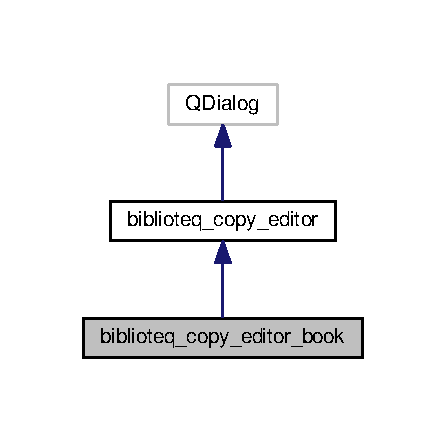
\includegraphics[width=214pt]{classbiblioteq__copy__editor__book__inherit__graph}
\end{center}
\end{figure}


Collaboration diagram for biblioteq\+\_\+copy\+\_\+editor\+\_\+book\+:
\nopagebreak
\begin{figure}[H]
\begin{center}
\leavevmode
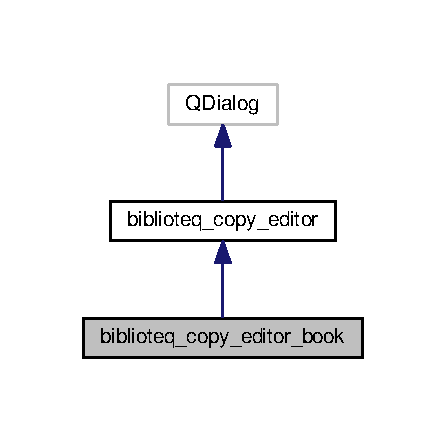
\includegraphics[width=214pt]{classbiblioteq__copy__editor__book__coll__graph}
\end{center}
\end{figure}
\subsection*{Public Member Functions}
\begin{DoxyCompactItemize}
\item 
{\bfseries biblioteq\+\_\+copy\+\_\+editor\+\_\+book} (Q\+Widget $\ast$parent, \hyperlink{classbiblioteq__item}{biblioteq\+\_\+item} $\ast$bitem\+Arg, const bool show\+For\+Lending\+Arg, const int quantity\+Arg, const Q\+String \&ioid\+Arg, Q\+Spin\+Box $\ast$spinbox\+Arg, const Q\+Font \&font, const Q\+String \&unique\+Id\+Arg)\hypertarget{classbiblioteq__copy__editor__book_aa232a71e2c3367aff273d0f5549db642}{}\label{classbiblioteq__copy__editor__book_aa232a71e2c3367aff273d0f5549db642}

\item 
void {\bfseries populate\+Copies\+Editor} (void)\hypertarget{classbiblioteq__copy__editor__book_a65d55067596ac47f73bee0ea9af3df31}{}\label{classbiblioteq__copy__editor__book_a65d55067596ac47f73bee0ea9af3df31}

\end{DoxyCompactItemize}
\subsection*{Additional Inherited Members}


The documentation for this class was generated from the following files\+:\begin{DoxyCompactItemize}
\item 
Source/biblioteq\+\_\+copy\+\_\+editor\+\_\+book.\+h\item 
Source/biblioteq\+\_\+copy\+\_\+editor\+\_\+book.\+cc\end{DoxyCompactItemize}

\hypertarget{classbiblioteq__dbenumerations}{}\section{biblioteq\+\_\+dbenumerations Class Reference}
\label{classbiblioteq__dbenumerations}\index{biblioteq\+\_\+dbenumerations@{biblioteq\+\_\+dbenumerations}}


Inheritance diagram for biblioteq\+\_\+dbenumerations\+:
\nopagebreak
\begin{figure}[H]
\begin{center}
\leavevmode
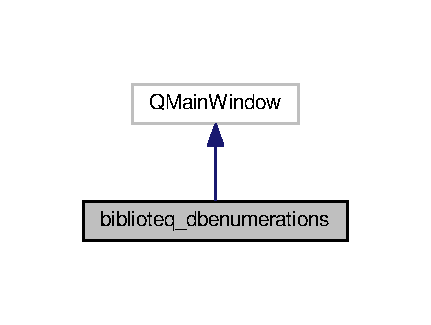
\includegraphics[width=207pt]{classbiblioteq__dbenumerations__inherit__graph}
\end{center}
\end{figure}


Collaboration diagram for biblioteq\+\_\+dbenumerations\+:
\nopagebreak
\begin{figure}[H]
\begin{center}
\leavevmode
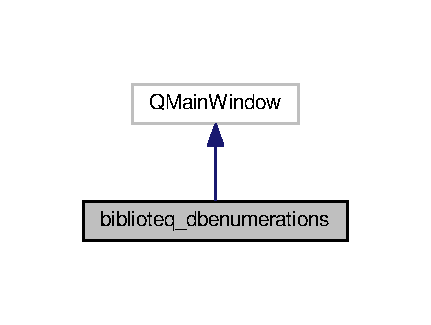
\includegraphics[width=207pt]{classbiblioteq__dbenumerations__coll__graph}
\end{center}
\end{figure}
\subsection*{Public Member Functions}
\begin{DoxyCompactItemize}
\item 
{\bfseries biblioteq\+\_\+dbenumerations} (Q\+Widget $\ast$parent)\hypertarget{classbiblioteq__dbenumerations_a7778f7dd99ba937b204f3ca6192bbe8e}{}\label{classbiblioteq__dbenumerations_a7778f7dd99ba937b204f3ca6192bbe8e}

\item 
void {\bfseries clear} (void)\hypertarget{classbiblioteq__dbenumerations_adccbde7a487bde517dca606889c2ec9a}{}\label{classbiblioteq__dbenumerations_adccbde7a487bde517dca606889c2ec9a}

\item 
void {\bfseries close\+Event} (Q\+Close\+Event $\ast$event)\hypertarget{classbiblioteq__dbenumerations_a39f3fd8a8b6244ed9598e47480a8b602}{}\label{classbiblioteq__dbenumerations_a39f3fd8a8b6244ed9598e47480a8b602}

\item 
void {\bfseries show} (Q\+Main\+Window $\ast$parent, const bool populate)\hypertarget{classbiblioteq__dbenumerations_a5c85f59659f447f0d921d3e8b6d461f8}{}\label{classbiblioteq__dbenumerations_a5c85f59659f447f0d921d3e8b6d461f8}

\end{DoxyCompactItemize}


The documentation for this class was generated from the following files\+:\begin{DoxyCompactItemize}
\item 
Source/biblioteq\+\_\+dbenumerations.\+h\item 
Source/biblioteq\+\_\+dbenumerations.\+cc\end{DoxyCompactItemize}

\hypertarget{classbiblioteq__dvd}{}\section{biblioteq\+\_\+dvd Class Reference}
\label{classbiblioteq__dvd}\index{biblioteq\+\_\+dvd@{biblioteq\+\_\+dvd}}


Inheritance diagram for biblioteq\+\_\+dvd\+:
\nopagebreak
\begin{figure}[H]
\begin{center}
\leavevmode
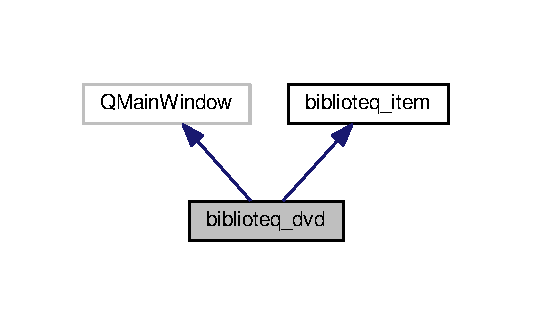
\includegraphics[width=256pt]{classbiblioteq__dvd__inherit__graph}
\end{center}
\end{figure}


Collaboration diagram for biblioteq\+\_\+dvd\+:
\nopagebreak
\begin{figure}[H]
\begin{center}
\leavevmode
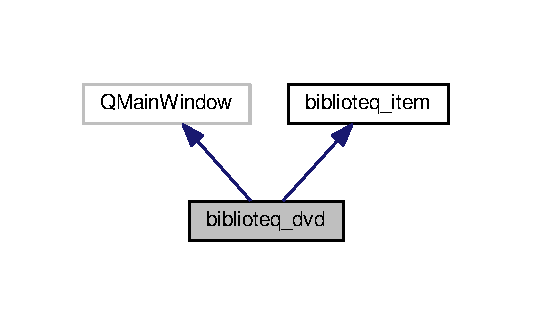
\includegraphics[width=256pt]{classbiblioteq__dvd__coll__graph}
\end{center}
\end{figure}
\subsection*{Public Member Functions}
\begin{DoxyCompactItemize}
\item 
{\bfseries biblioteq\+\_\+dvd} (Q\+Main\+Window $\ast$parent\+Arg, const Q\+String \&oid\+Arg, const int row\+Arg)\hypertarget{classbiblioteq__dvd_a44de06a196980a0b24a6a620e3f749f4}{}\label{classbiblioteq__dvd_a44de06a196980a0b24a6a620e3f749f4}

\item 
void {\bfseries duplicate} (const Q\+String \&p\+\_\+oid, const int state)\hypertarget{classbiblioteq__dvd_a2527917b6f26e1203c517e80d60df0ed}{}\label{classbiblioteq__dvd_a2527917b6f26e1203c517e80d60df0ed}

\item 
void {\bfseries insert} (void)\hypertarget{classbiblioteq__dvd_a5f7f1f5f37f8da30e52ae0d986fde626}{}\label{classbiblioteq__dvd_a5f7f1f5f37f8da30e52ae0d986fde626}

\item 
void {\bfseries modify} (const int state)\hypertarget{classbiblioteq__dvd_a5bea8b536366fa78954a32d10eb24249}{}\label{classbiblioteq__dvd_a5bea8b536366fa78954a32d10eb24249}

\item 
void {\bfseries search} (const Q\+String \&field=\char`\"{}\char`\"{}, const Q\+String \&value=\char`\"{}\char`\"{})\hypertarget{classbiblioteq__dvd_a21940a774debc4999ef1a8bec7f9af7a}{}\label{classbiblioteq__dvd_a21940a774debc4999ef1a8bec7f9af7a}

\item 
void {\bfseries set\+Publication\+Date\+Format} (const Q\+String \&date\+Format)\hypertarget{classbiblioteq__dvd_a7b15ae7b5eed23e998897b3fc294f3c3}{}\label{classbiblioteq__dvd_a7b15ae7b5eed23e998897b3fc294f3c3}

\item 
void {\bfseries update\+Window} (const int state)\hypertarget{classbiblioteq__dvd_ab93de53c2fd445a7209086e5126f55b7}{}\label{classbiblioteq__dvd_ab93de53c2fd445a7209086e5126f55b7}

\end{DoxyCompactItemize}
\subsection*{Additional Inherited Members}


The documentation for this class was generated from the following files\+:\begin{DoxyCompactItemize}
\item 
Source/biblioteq\+\_\+dvd.\+h\item 
Source/biblioteq\+\_\+dvd.\+cc\end{DoxyCompactItemize}

\hypertarget{classbiblioteq__generic__thread}{}\section{biblioteq\+\_\+generic\+\_\+thread Class Reference}
\label{classbiblioteq__generic__thread}\index{biblioteq\+\_\+generic\+\_\+thread@{biblioteq\+\_\+generic\+\_\+thread}}


Inheritance diagram for biblioteq\+\_\+generic\+\_\+thread\+:
\nopagebreak
\begin{figure}[H]
\begin{center}
\leavevmode
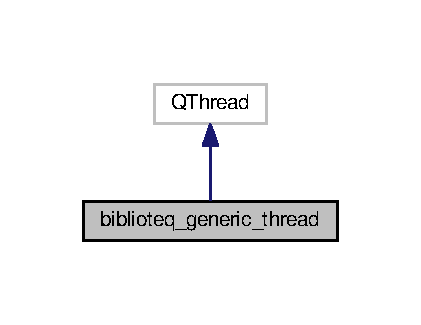
\includegraphics[width=202pt]{classbiblioteq__generic__thread__inherit__graph}
\end{center}
\end{figure}


Collaboration diagram for biblioteq\+\_\+generic\+\_\+thread\+:
\nopagebreak
\begin{figure}[H]
\begin{center}
\leavevmode
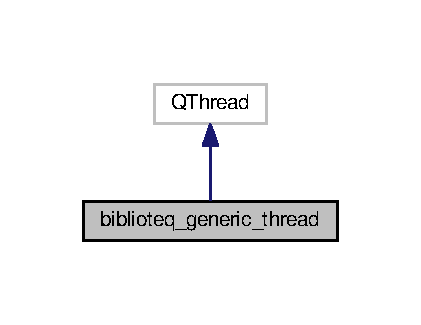
\includegraphics[width=202pt]{classbiblioteq__generic__thread__coll__graph}
\end{center}
\end{figure}
\subsection*{Public Member Functions}
\begin{DoxyCompactItemize}
\item 
{\bfseries biblioteq\+\_\+generic\+\_\+thread} (Q\+Object $\ast$parent)\hypertarget{classbiblioteq__generic__thread_aba1b257af43aafe990cf012928628d2b}{}\label{classbiblioteq__generic__thread_aba1b257af43aafe990cf012928628d2b}

\item 
Q\+String {\bfseries get\+E\+Type} (void) const \hypertarget{classbiblioteq__generic__thread_aeb37767f6fcb34a1345a889e00e8a072}{}\label{classbiblioteq__generic__thread_aeb37767f6fcb34a1345a889e00e8a072}

\item 
Q\+String {\bfseries get\+Error\+Str} (void) const \hypertarget{classbiblioteq__generic__thread_a5c8bfa2834af961976e01150a34142fd}{}\label{classbiblioteq__generic__thread_a5c8bfa2834af961976e01150a34142fd}

\item 
Q\+String\+List {\bfseries get\+List} (void) const \hypertarget{classbiblioteq__generic__thread_a191e577716aca59e7329c4ae4f00cf96}{}\label{classbiblioteq__generic__thread_a191e577716aca59e7329c4ae4f00cf96}

\item 
Q\+String\+List {\bfseries get\+Z3950\+Results} (void) const \hypertarget{classbiblioteq__generic__thread_aca4e1283cc3941ceb723ce7b344792b8}{}\label{classbiblioteq__generic__thread_aca4e1283cc3941ceb723ce7b344792b8}

\item 
void {\bfseries msleep} (const int msecs)\hypertarget{classbiblioteq__generic__thread_a4606ad74dd05e6fbfc561bfb43cdd521}{}\label{classbiblioteq__generic__thread_a4606ad74dd05e6fbfc561bfb43cdd521}

\item 
void {\bfseries run} (void)\hypertarget{classbiblioteq__generic__thread_a02ab41780ec4bb298d13fe2738d75a59}{}\label{classbiblioteq__generic__thread_a02ab41780ec4bb298d13fe2738d75a59}

\item 
void {\bfseries set\+Filename} (const Q\+String \&filename)\hypertarget{classbiblioteq__generic__thread_af04acb7ed95a2e374a5602b444f66589}{}\label{classbiblioteq__generic__thread_af04acb7ed95a2e374a5602b444f66589}

\item 
void {\bfseries set\+Output\+List} (const Q\+List$<$ bool $>$ \&list)\hypertarget{classbiblioteq__generic__thread_a2359d6a207d8371950c401943fdccfb5}{}\label{classbiblioteq__generic__thread_a2359d6a207d8371950c401943fdccfb5}

\item 
void {\bfseries set\+Type} (const int type)\hypertarget{classbiblioteq__generic__thread_a4b131d5b5c10ccd37ad661942901c4bb}{}\label{classbiblioteq__generic__thread_a4b131d5b5c10ccd37ad661942901c4bb}

\item 
void {\bfseries set\+Z3950\+Name} (const Q\+String \&name)\hypertarget{classbiblioteq__generic__thread_ac2b8101dbdb8a88a26e6cdac2d6eba3d}{}\label{classbiblioteq__generic__thread_ac2b8101dbdb8a88a26e6cdac2d6eba3d}

\item 
void {\bfseries set\+Z3950\+Search\+String} (const Q\+String \&z3950\+Search\+Str)\hypertarget{classbiblioteq__generic__thread_a0cc89d4c9c91da393e9970d6630f7b13}{}\label{classbiblioteq__generic__thread_a0cc89d4c9c91da393e9970d6630f7b13}

\end{DoxyCompactItemize}
\subsection*{Static Public Attributes}
\begin{DoxyCompactItemize}
\item 
static const int {\bfseries R\+E\+A\+D\+\_\+\+G\+L\+O\+B\+A\+L\+\_\+\+C\+O\+N\+F\+I\+G\+\_\+\+F\+I\+LE} = 200\hypertarget{classbiblioteq__generic__thread_a71ba3bd3edb966a8fae757d9f9190afa}{}\label{classbiblioteq__generic__thread_a71ba3bd3edb966a8fae757d9f9190afa}

\item 
static const int {\bfseries Z3950\+\_\+\+Q\+U\+E\+RY} = 300\hypertarget{classbiblioteq__generic__thread_a27d3813d7a948e36d540984c0f10512c}{}\label{classbiblioteq__generic__thread_a27d3813d7a948e36d540984c0f10512c}

\end{DoxyCompactItemize}


The documentation for this class was generated from the following files\+:\begin{DoxyCompactItemize}
\item 
Source/biblioteq\+\_\+generic\+\_\+thread.\+h\item 
Source/biblioteq\+\_\+generic\+\_\+thread.\+cc\end{DoxyCompactItemize}

\hypertarget{classbiblioteq__graphicsitempixmap}{}\section{biblioteq\+\_\+graphicsitempixmap Class Reference}
\label{classbiblioteq__graphicsitempixmap}\index{biblioteq\+\_\+graphicsitempixmap@{biblioteq\+\_\+graphicsitempixmap}}


Inheritance diagram for biblioteq\+\_\+graphicsitempixmap\+:
\nopagebreak
\begin{figure}[H]
\begin{center}
\leavevmode
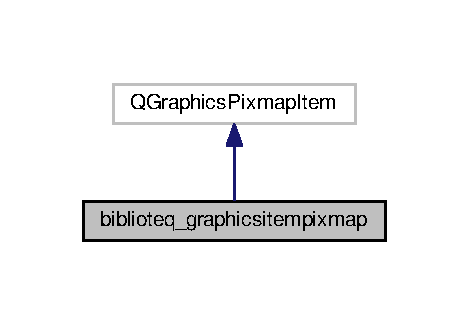
\includegraphics[width=225pt]{classbiblioteq__graphicsitempixmap__inherit__graph}
\end{center}
\end{figure}


Collaboration diagram for biblioteq\+\_\+graphicsitempixmap\+:
\nopagebreak
\begin{figure}[H]
\begin{center}
\leavevmode
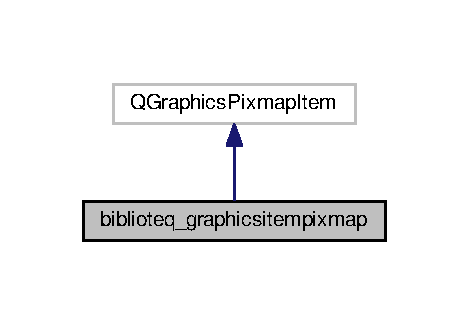
\includegraphics[width=225pt]{classbiblioteq__graphicsitempixmap__coll__graph}
\end{center}
\end{figure}
\subsection*{Public Member Functions}
\begin{DoxyCompactItemize}
\item 
{\bfseries biblioteq\+\_\+graphicsitempixmap} (const Q\+Pixmap \&pixmap, Q\+Graphics\+Item $\ast$parent)\hypertarget{classbiblioteq__graphicsitempixmap_a32d4d2f606c7043c500ba174bcea710b}{}\label{classbiblioteq__graphicsitempixmap_a32d4d2f606c7043c500ba174bcea710b}

\item 
void {\bfseries paint} (Q\+Painter $\ast$painter, const Q\+Style\+Option\+Graphics\+Item $\ast$option, Q\+Widget $\ast$widget=0)\hypertarget{classbiblioteq__graphicsitempixmap_a4518dd486c216bf46888ee6a91301067}{}\label{classbiblioteq__graphicsitempixmap_a4518dd486c216bf46888ee6a91301067}

\end{DoxyCompactItemize}


The documentation for this class was generated from the following file\+:\begin{DoxyCompactItemize}
\item 
Source/biblioteq\+\_\+graphicsitempixmap.\+h\end{DoxyCompactItemize}

\hypertarget{classbiblioteq__hyperlinked__text__edit}{}\section{biblioteq\+\_\+hyperlinked\+\_\+text\+\_\+edit Class Reference}
\label{classbiblioteq__hyperlinked__text__edit}\index{biblioteq\+\_\+hyperlinked\+\_\+text\+\_\+edit@{biblioteq\+\_\+hyperlinked\+\_\+text\+\_\+edit}}


Inheritance diagram for biblioteq\+\_\+hyperlinked\+\_\+text\+\_\+edit\+:
\nopagebreak
\begin{figure}[H]
\begin{center}
\leavevmode
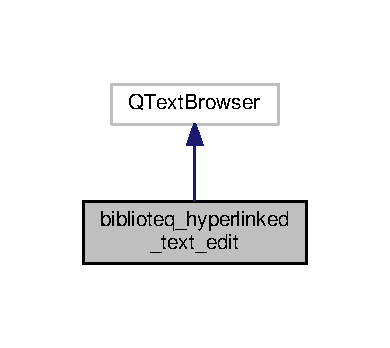
\includegraphics[width=187pt]{classbiblioteq__hyperlinked__text__edit__inherit__graph}
\end{center}
\end{figure}


Collaboration diagram for biblioteq\+\_\+hyperlinked\+\_\+text\+\_\+edit\+:
\nopagebreak
\begin{figure}[H]
\begin{center}
\leavevmode
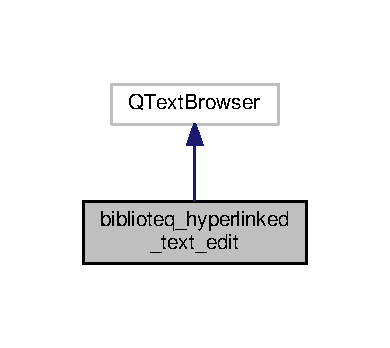
\includegraphics[width=187pt]{classbiblioteq__hyperlinked__text__edit__coll__graph}
\end{center}
\end{figure}
\subsection*{Public Member Functions}
\begin{DoxyCompactItemize}
\item 
{\bfseries biblioteq\+\_\+hyperlinked\+\_\+text\+\_\+edit} (Q\+Widget $\ast$parent)\hypertarget{classbiblioteq__hyperlinked__text__edit_a0341be34b832ac836f622a075b4e65c6}{}\label{classbiblioteq__hyperlinked__text__edit_a0341be34b832ac836f622a075b4e65c6}

\item 
void {\bfseries set\+Multiple\+Links} (const Q\+String \&search\+Type, const Q\+String \&search\+Field, const Q\+String \&str)\hypertarget{classbiblioteq__hyperlinked__text__edit_a80fe7ccc07d4d3559979db6dd128dd54}{}\label{classbiblioteq__hyperlinked__text__edit_a80fe7ccc07d4d3559979db6dd128dd54}

\end{DoxyCompactItemize}


The documentation for this class was generated from the following files\+:\begin{DoxyCompactItemize}
\item 
Source/biblioteq\+\_\+hyperlinked\+\_\+text\+\_\+edit.\+h\item 
Source/biblioteq\+\_\+hyperlinked\+\_\+text\+\_\+edit.\+cc\end{DoxyCompactItemize}

\hypertarget{classbiblioteq__image__drop__site}{}\section{biblioteq\+\_\+image\+\_\+drop\+\_\+site Class Reference}
\label{classbiblioteq__image__drop__site}\index{biblioteq\+\_\+image\+\_\+drop\+\_\+site@{biblioteq\+\_\+image\+\_\+drop\+\_\+site}}


Inheritance diagram for biblioteq\+\_\+image\+\_\+drop\+\_\+site\+:
\nopagebreak
\begin{figure}[H]
\begin{center}
\leavevmode
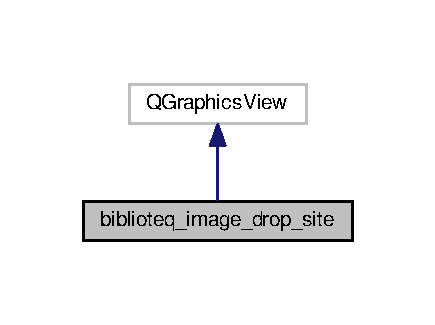
\includegraphics[width=209pt]{classbiblioteq__image__drop__site__inherit__graph}
\end{center}
\end{figure}


Collaboration diagram for biblioteq\+\_\+image\+\_\+drop\+\_\+site\+:
\nopagebreak
\begin{figure}[H]
\begin{center}
\leavevmode
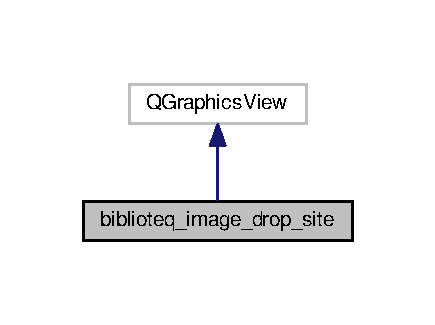
\includegraphics[width=209pt]{classbiblioteq__image__drop__site__coll__graph}
\end{center}
\end{figure}
\subsection*{Public Member Functions}
\begin{DoxyCompactItemize}
\item 
{\bfseries biblioteq\+\_\+image\+\_\+drop\+\_\+site} (Q\+Widget $\ast$parent)\hypertarget{classbiblioteq__image__drop__site_a530396fa05966eb322bd2a1125532ebf}{}\label{classbiblioteq__image__drop__site_a530396fa05966eb322bd2a1125532ebf}

\item 
void {\bfseries clear} (void)\hypertarget{classbiblioteq__image__drop__site_a3f88c28148dd3e47c928f90d19eb2602}{}\label{classbiblioteq__image__drop__site_a3f88c28148dd3e47c928f90d19eb2602}

\item 
void {\bfseries enable\+Double\+Click\+Resize} (const bool state)\hypertarget{classbiblioteq__image__drop__site_aa8ba78c79428c3347991a232d62b264a}{}\label{classbiblioteq__image__drop__site_aa8ba78c79428c3347991a232d62b264a}

\item 
void {\bfseries load\+From\+Data} (const Q\+Byte\+Array \&bytes)\hypertarget{classbiblioteq__image__drop__site_aaacb5dbb12a5e52402ebe21f9ca3dbb2}{}\label{classbiblioteq__image__drop__site_aaacb5dbb12a5e52402ebe21f9ca3dbb2}

\item 
void {\bfseries set\+Image} (const Q\+Image \&image)\hypertarget{classbiblioteq__image__drop__site_a40f01c405eb0b059d20cc46638c6f56c}{}\label{classbiblioteq__image__drop__site_a40f01c405eb0b059d20cc46638c6f56c}

\item 
void {\bfseries set\+Read\+Only} (const bool read\+Only)\hypertarget{classbiblioteq__image__drop__site_a4ea797056a2a0807e9acac0398b66422}{}\label{classbiblioteq__image__drop__site_a4ea797056a2a0807e9acac0398b66422}

\end{DoxyCompactItemize}
\subsection*{Public Attributes}
\begin{DoxyCompactItemize}
\item 
Q\+Image {\bfseries m\+\_\+image}\hypertarget{classbiblioteq__image__drop__site_a882e23b5ec4c5553a000c6a0811143bc}{}\label{classbiblioteq__image__drop__site_a882e23b5ec4c5553a000c6a0811143bc}

\item 
Q\+String {\bfseries m\+\_\+image\+Format}\hypertarget{classbiblioteq__image__drop__site_acebc24331f34bd5b4b7e4403e89f812b}{}\label{classbiblioteq__image__drop__site_acebc24331f34bd5b4b7e4403e89f812b}

\end{DoxyCompactItemize}


The documentation for this class was generated from the following files\+:\begin{DoxyCompactItemize}
\item 
Source/biblioteq\+\_\+image\+\_\+drop\+\_\+site.\+h\item 
Source/biblioteq\+\_\+image\+\_\+drop\+\_\+site.\+cc\end{DoxyCompactItemize}

\hypertarget{classbiblioteq__item}{}\section{biblioteq\+\_\+item Class Reference}
\label{classbiblioteq__item}\index{biblioteq\+\_\+item@{biblioteq\+\_\+item}}


Inheritance diagram for biblioteq\+\_\+item\+:
\nopagebreak
\begin{figure}[H]
\begin{center}
\leavevmode
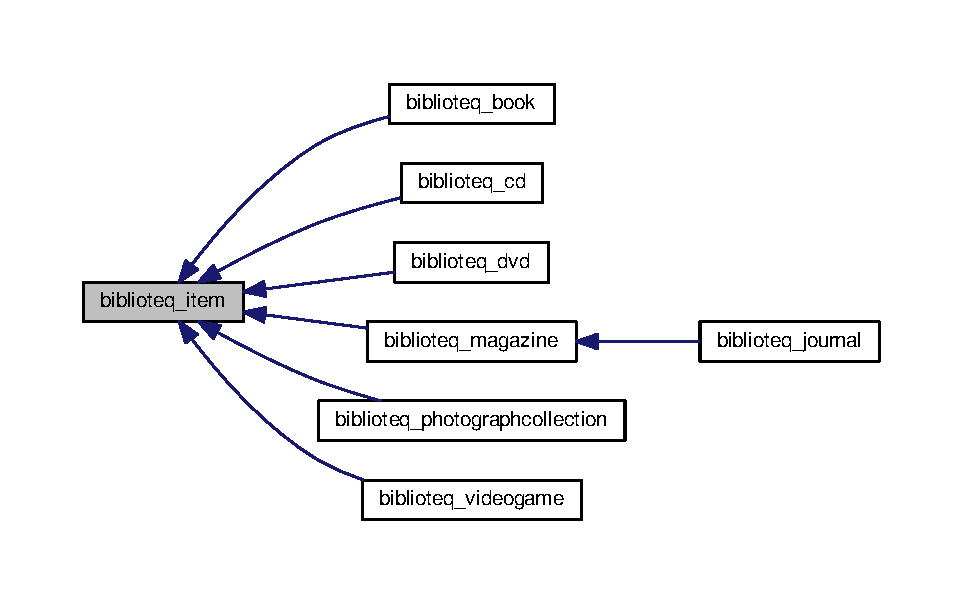
\includegraphics[width=350pt]{classbiblioteq__item__inherit__graph}
\end{center}
\end{figure}
\subsection*{Public Member Functions}
\begin{DoxyCompactItemize}
\item 
{\bfseries biblioteq\+\_\+item} (const int row\+Arg)\hypertarget{classbiblioteq__item_afe49e830ffa3c588e0f86f408ed09583}{}\label{classbiblioteq__item_afe49e830ffa3c588e0f86f408ed09583}

\item 
Q\+String {\bfseries get\+ID} (void) const \hypertarget{classbiblioteq__item_aa0e32c2b468b0ed6ff41915b71b4d8e4}{}\label{classbiblioteq__item_aa0e32c2b468b0ed6ff41915b71b4d8e4}

\item 
int {\bfseries get\+OldQ} (void) const \hypertarget{classbiblioteq__item_a6a23bf8eea0a6946dde80e3b33613438}{}\label{classbiblioteq__item_a6a23bf8eea0a6946dde80e3b33613438}

\item 
int {\bfseries get\+Row} (void) const \hypertarget{classbiblioteq__item_a14d2cc81d091747747094f78706f63b7}{}\label{classbiblioteq__item_a14d2cc81d091747747094f78706f63b7}

\item 
void {\bfseries set\+OldQ} (const int q)\hypertarget{classbiblioteq__item_ad234550506fe3daf2d1c2575d93427f0}{}\label{classbiblioteq__item_ad234550506fe3daf2d1c2575d93427f0}

\item 
void {\bfseries update\+Font} (const Q\+Font \&font, Q\+Widget $\ast$window)\hypertarget{classbiblioteq__item_ae66f8a9c95dbca54c1f8676853b813ac}{}\label{classbiblioteq__item_ae66f8a9c95dbca54c1f8676853b813ac}

\item 
void {\bfseries update\+Row} (const int row\+Arg)\hypertarget{classbiblioteq__item_a17b0313788c92a30a5bcd866c1266c54}{}\label{classbiblioteq__item_a17b0313788c92a30a5bcd866c1266c54}

\end{DoxyCompactItemize}
\subsection*{Protected Member Functions}
\begin{DoxyCompactItemize}
\item 
bool {\bfseries has\+Data\+Changed} (Q\+Main\+Window $\ast$window) const \hypertarget{classbiblioteq__item_aa4b679e9cc80339e07f50180986d04fc}{}\label{classbiblioteq__item_aa4b679e9cc80339e07f50180986d04fc}

\item 
void {\bfseries print} (Q\+Widget $\ast$parent)\hypertarget{classbiblioteq__item_a378140b7c2184e0efc743aa090780d5b}{}\label{classbiblioteq__item_a378140b7c2184e0efc743aa090780d5b}

\item 
void {\bfseries store\+Data} (Q\+Main\+Window $\ast$window)\hypertarget{classbiblioteq__item_a0d7b2b9d5079d2c0c979c44f0f71ad04}{}\label{classbiblioteq__item_a0d7b2b9d5079d2c0c979c44f0f71ad04}

\end{DoxyCompactItemize}
\subsection*{Protected Attributes}
\begin{DoxyCompactItemize}
\item 
Q\+Main\+Window $\ast$ {\bfseries m\+\_\+parent\+Wid}\hypertarget{classbiblioteq__item_aa90391a905a672a1943b93bf05d2aa60}{}\label{classbiblioteq__item_aa90391a905a672a1943b93bf05d2aa60}

\item 
Q\+Map$<$ Q\+String, Q\+Image $>$ {\bfseries m\+\_\+image\+Values}\hypertarget{classbiblioteq__item_a9bae246902c0170277c03663c6aec2cc}{}\label{classbiblioteq__item_a9bae246902c0170277c03663c6aec2cc}

\item 
Q\+Map$<$ Q\+String, Q\+String $>$ {\bfseries m\+\_\+widget\+Values}\hypertarget{classbiblioteq__item_a1fc18aef2f077ba7b6e872a50ba34b24}{}\label{classbiblioteq__item_a1fc18aef2f077ba7b6e872a50ba34b24}

\item 
Q\+String {\bfseries m\+\_\+html}\hypertarget{classbiblioteq__item_a1c79543a0d8070ff5e143791275d332c}{}\label{classbiblioteq__item_a1c79543a0d8070ff5e143791275d332c}

\item 
Q\+String {\bfseries m\+\_\+oid}\hypertarget{classbiblioteq__item_a154463dc3fe45fe19b055e4361ee3f78}{}\label{classbiblioteq__item_a154463dc3fe45fe19b055e4361ee3f78}

\item 
bool {\bfseries m\+\_\+is\+Query\+Enabled}\hypertarget{classbiblioteq__item_ae7e4923f4e6c809f3480dcf3583a00e1}{}\label{classbiblioteq__item_ae7e4923f4e6c809f3480dcf3583a00e1}

\item 
int {\bfseries m\+\_\+oldq}\hypertarget{classbiblioteq__item_a1e969ab09e319001a6d8d709e8f80d0c}{}\label{classbiblioteq__item_a1e969ab09e319001a6d8d709e8f80d0c}

\item 
int {\bfseries m\+\_\+row}\hypertarget{classbiblioteq__item_a638cf673c669e8f11e219289917617bd}{}\label{classbiblioteq__item_a638cf673c669e8f11e219289917617bd}

\end{DoxyCompactItemize}


The documentation for this class was generated from the following files\+:\begin{DoxyCompactItemize}
\item 
Source/biblioteq\+\_\+item.\+h\item 
Source/biblioteq\+\_\+item.\+cc\end{DoxyCompactItemize}

\hypertarget{classbiblioteq__item__working__dialog}{}\section{biblioteq\+\_\+item\+\_\+working\+\_\+dialog Class Reference}
\label{classbiblioteq__item__working__dialog}\index{biblioteq\+\_\+item\+\_\+working\+\_\+dialog@{biblioteq\+\_\+item\+\_\+working\+\_\+dialog}}


Inheritance diagram for biblioteq\+\_\+item\+\_\+working\+\_\+dialog\+:
\nopagebreak
\begin{figure}[H]
\begin{center}
\leavevmode
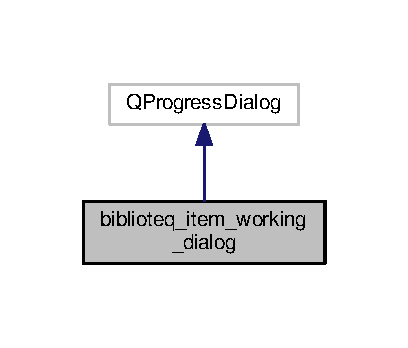
\includegraphics[width=196pt]{classbiblioteq__item__working__dialog__inherit__graph}
\end{center}
\end{figure}


Collaboration diagram for biblioteq\+\_\+item\+\_\+working\+\_\+dialog\+:
\nopagebreak
\begin{figure}[H]
\begin{center}
\leavevmode
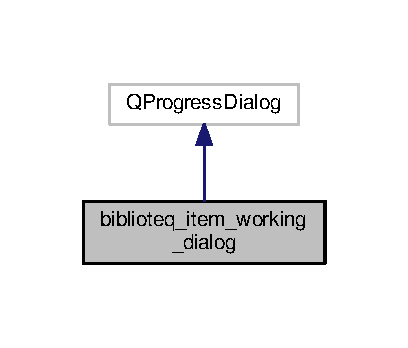
\includegraphics[width=196pt]{classbiblioteq__item__working__dialog__coll__graph}
\end{center}
\end{figure}
\subsection*{Public Member Functions}
\begin{DoxyCompactItemize}
\item 
{\bfseries biblioteq\+\_\+item\+\_\+working\+\_\+dialog} (Q\+Main\+Window $\ast$parent)\hypertarget{classbiblioteq__item__working__dialog_aabd2c6535a5e68ea8c0be9fa1ebaa6a8}{}\label{classbiblioteq__item__working__dialog_aabd2c6535a5e68ea8c0be9fa1ebaa6a8}

\end{DoxyCompactItemize}
\subsection*{Protected Member Functions}
\begin{DoxyCompactItemize}
\item 
void {\bfseries close\+Event} (Q\+Close\+Event $\ast$event)\hypertarget{classbiblioteq__item__working__dialog_a4e79bf3607bf6190d2a5ab1f15100bf6}{}\label{classbiblioteq__item__working__dialog_a4e79bf3607bf6190d2a5ab1f15100bf6}

\item 
void {\bfseries key\+Press\+Event} (Q\+Key\+Event $\ast$event)\hypertarget{classbiblioteq__item__working__dialog_a64373b8f8319ad379ae7309f83ff61d4}{}\label{classbiblioteq__item__working__dialog_a64373b8f8319ad379ae7309f83ff61d4}

\end{DoxyCompactItemize}


The documentation for this class was generated from the following file\+:\begin{DoxyCompactItemize}
\item 
Source/biblioteq\+\_\+item.\+h\end{DoxyCompactItemize}

\hypertarget{classbiblioteq__journal}{}\section{biblioteq\+\_\+journal Class Reference}
\label{classbiblioteq__journal}\index{biblioteq\+\_\+journal@{biblioteq\+\_\+journal}}


Inheritance diagram for biblioteq\+\_\+journal\+:
\nopagebreak
\begin{figure}[H]
\begin{center}
\leavevmode
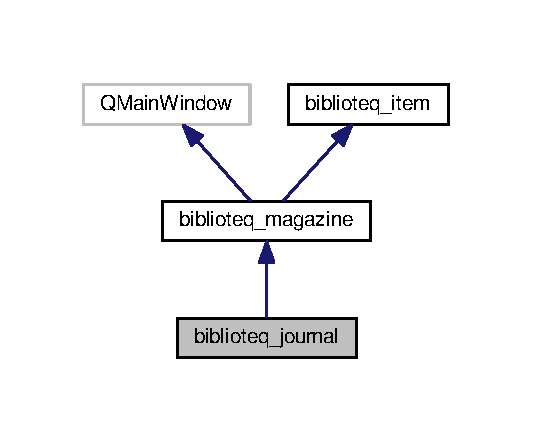
\includegraphics[width=256pt]{classbiblioteq__journal__inherit__graph}
\end{center}
\end{figure}


Collaboration diagram for biblioteq\+\_\+journal\+:
\nopagebreak
\begin{figure}[H]
\begin{center}
\leavevmode
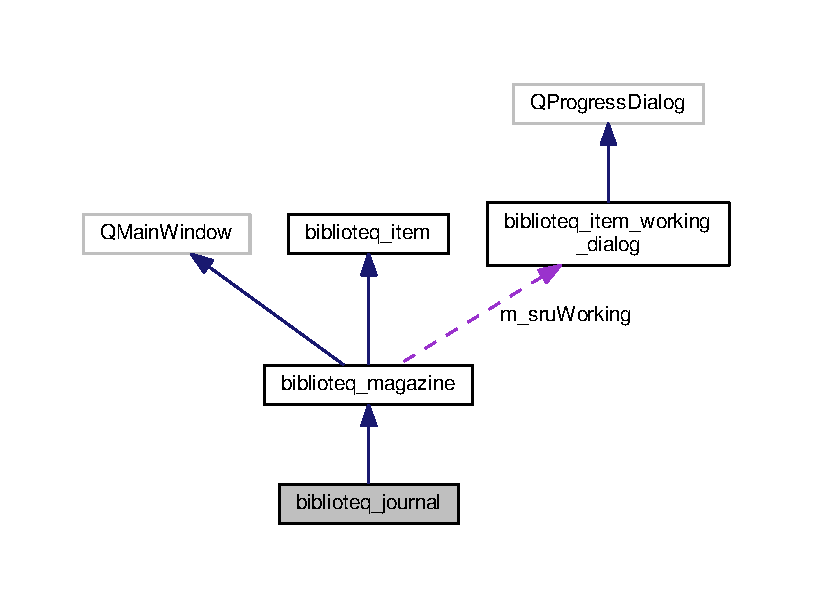
\includegraphics[width=350pt]{classbiblioteq__journal__coll__graph}
\end{center}
\end{figure}
\subsection*{Public Member Functions}
\begin{DoxyCompactItemize}
\item 
{\bfseries biblioteq\+\_\+journal} (Q\+Main\+Window $\ast$parent\+Arg, const Q\+String \&oid\+Arg, const int row\+Arg)\hypertarget{classbiblioteq__journal_a38aed34a81ec9d4e28461bf430df9d3e}{}\label{classbiblioteq__journal_a38aed34a81ec9d4e28461bf430df9d3e}

\item 
void {\bfseries change\+Event} (Q\+Event $\ast$event)\hypertarget{classbiblioteq__journal_a8ad8e85e674b7a5012d71a49fe9e6eee}{}\label{classbiblioteq__journal_a8ad8e85e674b7a5012d71a49fe9e6eee}

\item 
void {\bfseries close\+Event} (Q\+Close\+Event $\ast$event)\hypertarget{classbiblioteq__journal_a0099d00efd5be69fb2632493d50b5838}{}\label{classbiblioteq__journal_a0099d00efd5be69fb2632493d50b5838}

\end{DoxyCompactItemize}
\subsection*{Additional Inherited Members}


The documentation for this class was generated from the following files\+:\begin{DoxyCompactItemize}
\item 
Source/biblioteq\+\_\+magazine.\+h\item 
Source/biblioteq\+\_\+journal.\+cc\end{DoxyCompactItemize}

\hypertarget{classbiblioteq__magazine}{}\section{biblioteq\+\_\+magazine Class Reference}
\label{classbiblioteq__magazine}\index{biblioteq\+\_\+magazine@{biblioteq\+\_\+magazine}}


Inheritance diagram for biblioteq\+\_\+magazine\+:
\nopagebreak
\begin{figure}[H]
\begin{center}
\leavevmode
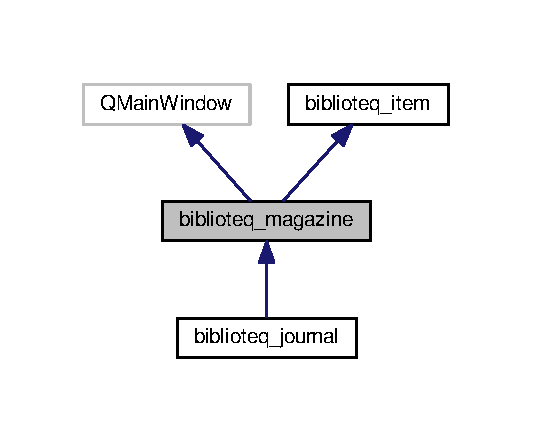
\includegraphics[width=256pt]{classbiblioteq__magazine__inherit__graph}
\end{center}
\end{figure}


Collaboration diagram for biblioteq\+\_\+magazine\+:
\nopagebreak
\begin{figure}[H]
\begin{center}
\leavevmode
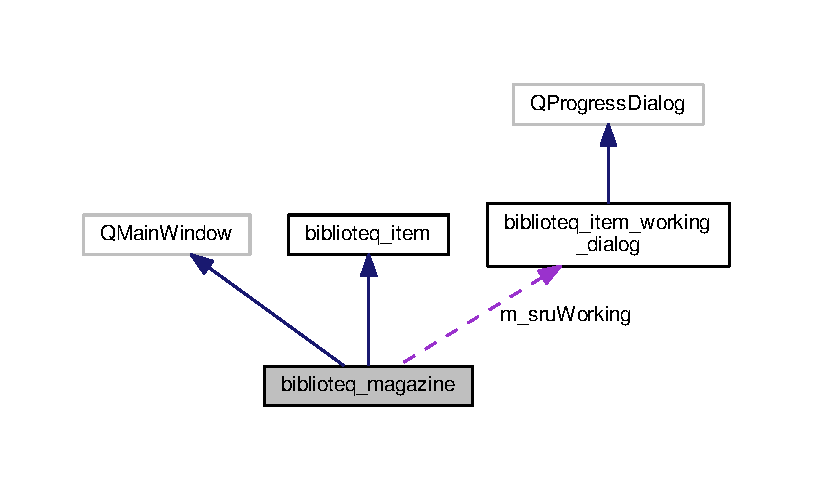
\includegraphics[width=350pt]{classbiblioteq__magazine__coll__graph}
\end{center}
\end{figure}
\subsection*{Public Member Functions}
\begin{DoxyCompactItemize}
\item 
{\bfseries biblioteq\+\_\+magazine} (Q\+Main\+Window $\ast$parent\+Arg, const Q\+String \&oid\+Arg, const int row\+Arg, const Q\+String \&sub\+Type\+Arg)\hypertarget{classbiblioteq__magazine_ad28113019caa57b7ee667a82516b7bef}{}\label{classbiblioteq__magazine_ad28113019caa57b7ee667a82516b7bef}

\item 
Ui\+\_\+mag\+Dialog {\bfseries dialog} (void) const \hypertarget{classbiblioteq__magazine_aefc3cf7d5dc6f2af91040d8ba681b6f3}{}\label{classbiblioteq__magazine_aefc3cf7d5dc6f2af91040d8ba681b6f3}

\item 
void {\bfseries duplicate} (const Q\+String \&p\+\_\+oid, const int state)\hypertarget{classbiblioteq__magazine_ac02b6ebcb65686082f8fb3ffa411288d}{}\label{classbiblioteq__magazine_ac02b6ebcb65686082f8fb3ffa411288d}

\item 
void {\bfseries insert} (void)\hypertarget{classbiblioteq__magazine_a28d4da5cc33f6ac02373b85dfe4240b7}{}\label{classbiblioteq__magazine_a28d4da5cc33f6ac02373b85dfe4240b7}

\item 
void {\bfseries modify} (const int)\hypertarget{classbiblioteq__magazine_a5a542d604cf17ca39bca7de932ffa248}{}\label{classbiblioteq__magazine_a5a542d604cf17ca39bca7de932ffa248}

\item 
void {\bfseries populate\+Display\+After\+S\+RU} (const Q\+Byte\+Array \&data)\hypertarget{classbiblioteq__magazine_a1140e43db1cad46da869287e29a2b523}{}\label{classbiblioteq__magazine_a1140e43db1cad46da869287e29a2b523}

\item 
void {\bfseries populate\+Display\+After\+Z3950} (const Q\+String\+List \&list, const Q\+String \&record\+Syntax)\hypertarget{classbiblioteq__magazine_a4bd4c1cb752ec7b0eab449e83a21056d}{}\label{classbiblioteq__magazine_a4bd4c1cb752ec7b0eab449e83a21056d}

\item 
void {\bfseries set\+Publication\+Date\+Format} (const Q\+String \&date\+Format)\hypertarget{classbiblioteq__magazine_aa7add0d8bcdf55402817d3d8be6e09c7}{}\label{classbiblioteq__magazine_aa7add0d8bcdf55402817d3d8be6e09c7}

\item 
void {\bfseries search} (const Q\+String \&field=\char`\"{}\char`\"{}, const Q\+String \&value=\char`\"{}\char`\"{})\hypertarget{classbiblioteq__magazine_af39a2b84bc3ee9d108812a9df2137bfc}{}\label{classbiblioteq__magazine_af39a2b84bc3ee9d108812a9df2137bfc}

\item 
void {\bfseries update\+Window} (const int state)\hypertarget{classbiblioteq__magazine_a5645500bca3c8cc4360ec1b75f1abd5b}{}\label{classbiblioteq__magazine_a5645500bca3c8cc4360ec1b75f1abd5b}

\end{DoxyCompactItemize}
\subsection*{Protected Slots}
\begin{DoxyCompactItemize}
\item 
void {\bfseries slot\+Attach\+Files} (void)\hypertarget{classbiblioteq__magazine_aac83be1223224e358440d5a5b928b263}{}\label{classbiblioteq__magazine_aac83be1223224e358440d5a5b928b263}

\item 
void {\bfseries slot\+Cancel} (void)\hypertarget{classbiblioteq__magazine_ac5808297f5976e5ef2883b90b04aaa03}{}\label{classbiblioteq__magazine_ac5808297f5976e5ef2883b90b04aaa03}

\item 
void {\bfseries slot\+Delete\+Files} (void)\hypertarget{classbiblioteq__magazine_accad672caf97ae20df3e9afb8aa8ae5a}{}\label{classbiblioteq__magazine_accad672caf97ae20df3e9afb8aa8ae5a}

\item 
void {\bfseries slot\+Edit\+File\+Description} (Q\+Table\+Widget\+Item $\ast$item)\hypertarget{classbiblioteq__magazine_a7d9634c005e3934a16f71812dd5f5439}{}\label{classbiblioteq__magazine_a7d9634c005e3934a16f71812dd5f5439}

\item 
void {\bfseries slot\+Export\+Files} (void)\hypertarget{classbiblioteq__magazine_a716eba32a5a26f2c5523d17f3edabfba}{}\label{classbiblioteq__magazine_a716eba32a5a26f2c5523d17f3edabfba}

\item 
void {\bfseries slot\+Go} (void)\hypertarget{classbiblioteq__magazine_a1faba8da2af2924afe2bdd726c27d530}{}\label{classbiblioteq__magazine_a1faba8da2af2924afe2bdd726c27d530}

\item 
void {\bfseries slot\+Populate\+Copies\+Editor} (void)\hypertarget{classbiblioteq__magazine_a14eb96b25a7f1369718bd2b97666beb1}{}\label{classbiblioteq__magazine_a14eb96b25a7f1369718bd2b97666beb1}

\item 
void {\bfseries slot\+Print} (void)\hypertarget{classbiblioteq__magazine_a9df9bd8bee01833709722ee547cc6006}{}\label{classbiblioteq__magazine_a9df9bd8bee01833709722ee547cc6006}

\item 
void {\bfseries slot\+Proxy\+Authentication\+Required} (const Q\+Network\+Proxy \&proxy, Q\+Authenticator $\ast$authenticator)\hypertarget{classbiblioteq__magazine_a255c2b2364d0f19a4fbe2434c7fee1e9}{}\label{classbiblioteq__magazine_a255c2b2364d0f19a4fbe2434c7fee1e9}

\item 
void {\bfseries slot\+Reset} (void)\hypertarget{classbiblioteq__magazine_aae07fff6d5119cfe2660b32858c5559a}{}\label{classbiblioteq__magazine_aae07fff6d5119cfe2660b32858c5559a}

\item 
void {\bfseries slot\+S\+R\+U\+Download\+Finished} (bool error)\hypertarget{classbiblioteq__magazine_a81dbe5bdf964c73d2495103f62407a5d}{}\label{classbiblioteq__magazine_a81dbe5bdf964c73d2495103f62407a5d}

\item 
void {\bfseries slot\+S\+R\+U\+Download\+Finished} (void)\hypertarget{classbiblioteq__magazine_a6c2166d6be894aaa884f498916e1876a}{}\label{classbiblioteq__magazine_a6c2166d6be894aaa884f498916e1876a}

\item 
void {\bfseries slot\+S\+R\+U\+Query} (void)\hypertarget{classbiblioteq__magazine_a3910676f5efa8718bb2e48df1ee49c7a}{}\label{classbiblioteq__magazine_a3910676f5efa8718bb2e48df1ee49c7a}

\item 
void {\bfseries slot\+S\+R\+U\+Ready\+Read} (const Q\+Http\+Response\+Header \&resp)\hypertarget{classbiblioteq__magazine_a7bd42577104b706a2a228cdd6070faa5}{}\label{classbiblioteq__magazine_a7bd42577104b706a2a228cdd6070faa5}

\item 
void {\bfseries slot\+S\+R\+U\+Ready\+Read} (void)\hypertarget{classbiblioteq__magazine_a7e00a4c73e3ffa3bde88e36d73fc94b8}{}\label{classbiblioteq__magazine_a7e00a4c73e3ffa3bde88e36d73fc94b8}

\item 
void {\bfseries slot\+Select\+Image} (void)\hypertarget{classbiblioteq__magazine_afa046729bc79d76f78f60f12231b71d1}{}\label{classbiblioteq__magazine_afa046729bc79d76f78f60f12231b71d1}

\item 
void {\bfseries slot\+Show\+P\+DF} (void)\hypertarget{classbiblioteq__magazine_aa1ca8fee6fcc8e0c09bcb593e944c940}{}\label{classbiblioteq__magazine_aa1ca8fee6fcc8e0c09bcb593e944c940}

\item 
void {\bfseries slot\+Show\+Users} (void)\hypertarget{classbiblioteq__magazine_a523c1274c25eeb93e76babe40b709c95}{}\label{classbiblioteq__magazine_a523c1274c25eeb93e76babe40b709c95}

\item 
void {\bfseries slot\+Z3950\+Query} (void)\hypertarget{classbiblioteq__magazine_a846f231c5809497ee8c173182faa3c61}{}\label{classbiblioteq__magazine_a846f231c5809497ee8c173182faa3c61}

\end{DoxyCompactItemize}
\subsection*{Protected Member Functions}
\begin{DoxyCompactItemize}
\item 
bool {\bfseries use\+Http} (void) const \hypertarget{classbiblioteq__magazine_a4417201ab4c6d0718580d3d48e6f2406}{}\label{classbiblioteq__magazine_a4417201ab4c6d0718580d3d48e6f2406}

\item 
void {\bfseries change\+Event} (Q\+Event $\ast$event)\hypertarget{classbiblioteq__magazine_a724764880bf4aed8878a6a43681faf3f}{}\label{classbiblioteq__magazine_a724764880bf4aed8878a6a43681faf3f}

\item 
void {\bfseries create\+File} (const Q\+Byte\+Array \&digest, const Q\+Byte\+Array \&bytes, const Q\+String \&file\+Name) const \hypertarget{classbiblioteq__magazine_ae1863bcd350f14146b7a6589157b2608}{}\label{classbiblioteq__magazine_ae1863bcd350f14146b7a6589157b2608}

\item 
void {\bfseries close\+Event} (Q\+Close\+Event $\ast$event)\hypertarget{classbiblioteq__magazine_a87f20b7fc43d1ea4fe1793112604f34a}{}\label{classbiblioteq__magazine_a87f20b7fc43d1ea4fe1793112604f34a}

\item 
void {\bfseries populate\+Files} (void)\hypertarget{classbiblioteq__magazine_aa314072fc48397808a82bbe49d378a56}{}\label{classbiblioteq__magazine_aa314072fc48397808a82bbe49d378a56}

\item 
void {\bfseries sru\+Download\+Finished} (void)\hypertarget{classbiblioteq__magazine_a0d651d79caeed52b2d2022e854adf027}{}\label{classbiblioteq__magazine_a0d651d79caeed52b2d2022e854adf027}

\end{DoxyCompactItemize}
\subsection*{Protected Attributes}
\begin{DoxyCompactItemize}
\item 
Q\+Byte\+Array {\bfseries m\+\_\+sru\+Results}\hypertarget{classbiblioteq__magazine_aa323a2c4ad4ced05d7c29e25dc737d35}{}\label{classbiblioteq__magazine_aa323a2c4ad4ced05d7c29e25dc737d35}

\item 
Q\+Dialog $\ast$ {\bfseries m\+\_\+proxy\+Dialog}\hypertarget{classbiblioteq__magazine_a9bc0a7a5e2037652659499a8b651ffbd}{}\label{classbiblioteq__magazine_a9bc0a7a5e2037652659499a8b651ffbd}

\item 
Q\+Http $\ast$ {\bfseries m\+\_\+sru\+Http}\hypertarget{classbiblioteq__magazine_a0edec00c791d597fad5c30e91b51f5fe}{}\label{classbiblioteq__magazine_a0edec00c791d597fad5c30e91b51f5fe}

\item 
Q\+Network\+Access\+Manager $\ast$ {\bfseries m\+\_\+sru\+Manager}\hypertarget{classbiblioteq__magazine_ad8141d59f535cf3d03476e5b1ac2aec4}{}\label{classbiblioteq__magazine_ad8141d59f535cf3d03476e5b1ac2aec4}

\item 
Q\+Palette {\bfseries m\+\_\+cb\+\_\+orig\+\_\+pal}\hypertarget{classbiblioteq__magazine_a12c0a24b9abfb1b9ff5a2e18678e4997}{}\label{classbiblioteq__magazine_a12c0a24b9abfb1b9ff5a2e18678e4997}

\item 
Q\+Palette {\bfseries m\+\_\+te\+\_\+orig\+\_\+pal}\hypertarget{classbiblioteq__magazine_a168b40414fedf417fe53d85bb0183455}{}\label{classbiblioteq__magazine_a168b40414fedf417fe53d85bb0183455}

\item 
Q\+Palette {\bfseries m\+\_\+white\+\_\+pal}\hypertarget{classbiblioteq__magazine_a1ac7f3617c7433be0a3b58995bb0a83f}{}\label{classbiblioteq__magazine_a1ac7f3617c7433be0a3b58995bb0a83f}

\item 
Q\+Pointer$<$ \hyperlink{classbiblioteq__generic__thread}{biblioteq\+\_\+generic\+\_\+thread} $>$ {\bfseries m\+\_\+thread}\hypertarget{classbiblioteq__magazine_a600a4c29510430526eae82bd7d11e246}{}\label{classbiblioteq__magazine_a600a4c29510430526eae82bd7d11e246}

\item 
Q\+String {\bfseries m\+\_\+dt\+\_\+orig\+\_\+ss}\hypertarget{classbiblioteq__magazine_a48689c815bab3c63e1b39af0ac966eeb}{}\label{classbiblioteq__magazine_a48689c815bab3c63e1b39af0ac966eeb}

\item 
Q\+String {\bfseries m\+\_\+eng\+Window\+Title}\hypertarget{classbiblioteq__magazine_a5ee1f5830c82adf6f9e2a01f1e9b084e}{}\label{classbiblioteq__magazine_a5ee1f5830c82adf6f9e2a01f1e9b084e}

\item 
Q\+String {\bfseries m\+\_\+sub\+Type}\hypertarget{classbiblioteq__magazine_a022e8b83ecf4c0d71d55b82f91aafc04}{}\label{classbiblioteq__magazine_a022e8b83ecf4c0d71d55b82f91aafc04}

\item 
Ui\+\_\+mag\+Dialog {\bfseries ma}\hypertarget{classbiblioteq__magazine_a2882fe0804626976a30c4276db27cf27}{}\label{classbiblioteq__magazine_a2882fe0804626976a30c4276db27cf27}

\item 
Ui\+\_\+password\+Dialog {\bfseries ui\+\_\+p}\hypertarget{classbiblioteq__magazine_ab158ab3dd515fa0b54d70da11cabd091}{}\label{classbiblioteq__magazine_ab158ab3dd515fa0b54d70da11cabd091}

\item 
\hyperlink{classbiblioteq__item__working__dialog}{biblioteq\+\_\+item\+\_\+working\+\_\+dialog} $\ast$ {\bfseries m\+\_\+sru\+Working}\hypertarget{classbiblioteq__magazine_aca999487ac2250ea5bcecd11ab9835b2}{}\label{classbiblioteq__magazine_aca999487ac2250ea5bcecd11ab9835b2}

\item 
bool {\bfseries m\+\_\+duplicate}\hypertarget{classbiblioteq__magazine_ac80146dd2c8a55cf4dcca59abca320d1}{}\label{classbiblioteq__magazine_ac80146dd2c8a55cf4dcca59abca320d1}

\end{DoxyCompactItemize}


The documentation for this class was generated from the following files\+:\begin{DoxyCompactItemize}
\item 
Source/biblioteq\+\_\+magazine.\+h\item 
Source/biblioteq\+\_\+magazine.\+cc\end{DoxyCompactItemize}

\hypertarget{classbiblioteq__main__table}{}\section{biblioteq\+\_\+main\+\_\+table Class Reference}
\label{classbiblioteq__main__table}\index{biblioteq\+\_\+main\+\_\+table@{biblioteq\+\_\+main\+\_\+table}}


Inheritance diagram for biblioteq\+\_\+main\+\_\+table\+:
\nopagebreak
\begin{figure}[H]
\begin{center}
\leavevmode
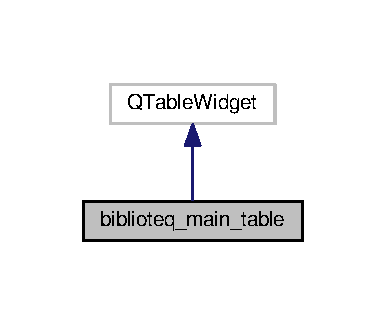
\includegraphics[width=185pt]{classbiblioteq__main__table__inherit__graph}
\end{center}
\end{figure}


Collaboration diagram for biblioteq\+\_\+main\+\_\+table\+:
\nopagebreak
\begin{figure}[H]
\begin{center}
\leavevmode
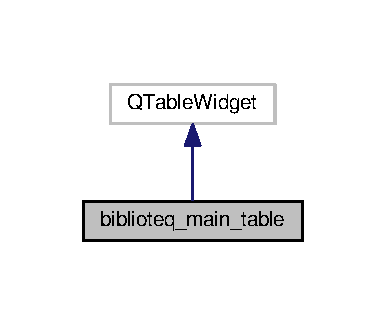
\includegraphics[width=185pt]{classbiblioteq__main__table__coll__graph}
\end{center}
\end{figure}
\subsection*{Public Member Functions}
\begin{DoxyCompactItemize}
\item 
{\bfseries biblioteq\+\_\+main\+\_\+table} (Q\+Widget $\ast$parent)\hypertarget{classbiblioteq__main__table_ab3c4f8fa63984fd571de87be8cf4e2ac}{}\label{classbiblioteq__main__table_ab3c4f8fa63984fd571de87be8cf4e2ac}

\item 
Q\+Hash$<$ Q\+String, Q\+String $>$ {\bfseries friendly\+States} (void) const \hypertarget{classbiblioteq__main__table_af5836fee6e018560a9fef97fe557bdb3}{}\label{classbiblioteq__main__table_af5836fee6e018560a9fef97fe557bdb3}

\item 
Q\+String\+List {\bfseries column\+Names} (void) const \hypertarget{classbiblioteq__main__table_aaf9a0b14625e0dd8ceaa1bfe0c54405f}{}\label{classbiblioteq__main__table_aaf9a0b14625e0dd8ceaa1bfe0c54405f}

\item 
int {\bfseries column\+Number} (const Q\+String \&name) const \hypertarget{classbiblioteq__main__table_ada630dc6d45bd2c1ae73889204a38353}{}\label{classbiblioteq__main__table_ada630dc6d45bd2c1ae73889204a38353}

\item 
void {\bfseries parse\+States} (const Q\+Hash$<$ Q\+String, Q\+String $>$ \&states)\hypertarget{classbiblioteq__main__table_a0035686c1a915aefe9ee89de443333c8}{}\label{classbiblioteq__main__table_a0035686c1a915aefe9ee89de443333c8}

\item 
void {\bfseries record\+Column\+Hidden} (const Q\+String \&username, const Q\+String \&type, const int index, const bool hidden)\hypertarget{classbiblioteq__main__table_a0a6a8ea89801929a45f86ca3cf1e3215}{}\label{classbiblioteq__main__table_a0a6a8ea89801929a45f86ca3cf1e3215}

\item 
void {\bfseries reset\+Table} (const Q\+String \&username, const Q\+String \&type, const Q\+String \&roles)\hypertarget{classbiblioteq__main__table_a5c447d10b414d68f4c5d4e052f718b01}{}\label{classbiblioteq__main__table_a5c447d10b414d68f4c5d4e052f718b01}

\item 
void {\bfseries set\+Column\+Names} (const Q\+String\+List \&list)\hypertarget{classbiblioteq__main__table_a8f0aba1cda6e577bd44b7854d813446a}{}\label{classbiblioteq__main__table_a8f0aba1cda6e577bd44b7854d813446a}

\end{DoxyCompactItemize}


The documentation for this class was generated from the following files\+:\begin{DoxyCompactItemize}
\item 
Source/biblioteq\+\_\+main\+\_\+table.\+h\item 
Source/biblioteq\+\_\+main\+\_\+table.\+cc\end{DoxyCompactItemize}

\hypertarget{classbiblioteq__marc}{}\section{biblioteq\+\_\+marc Class Reference}
\label{classbiblioteq__marc}\index{biblioteq\+\_\+marc@{biblioteq\+\_\+marc}}
\subsection*{Public Types}
\begin{DoxyCompactItemize}
\item 
enum {\bfseries I\+T\+E\+M\+\_\+\+T\+Y\+PE} \{ {\bfseries B\+O\+OK} = 0, 
{\bfseries M\+A\+G\+A\+Z\+I\+NE}
 \}\hypertarget{classbiblioteq__marc_aef55c45eeca365be310533f0c318c877}{}\label{classbiblioteq__marc_aef55c45eeca365be310533f0c318c877}

\item 
enum {\bfseries P\+R\+O\+T\+O\+C\+OL} \{ {\bfseries S\+RU} = 0, 
{\bfseries Z3950}
 \}\hypertarget{classbiblioteq__marc_ae2e5c435b3e42f74d9a58ce2a17907ef}{}\label{classbiblioteq__marc_ae2e5c435b3e42f74d9a58ce2a17907ef}

\item 
enum {\bfseries R\+E\+C\+O\+R\+D\+\_\+\+S\+Y\+N\+T\+AX} \{ {\bfseries M\+A\+R\+C21} = 0, 
{\bfseries U\+N\+I\+M\+A\+RC}
 \}\hypertarget{classbiblioteq__marc_af1bcc8df3efe413864deb128541b8264}{}\label{classbiblioteq__marc_af1bcc8df3efe413864deb128541b8264}

\end{DoxyCompactItemize}
\subsection*{Public Member Functions}
\begin{DoxyCompactItemize}
\item 
{\bfseries biblioteq\+\_\+marc} (const I\+T\+E\+M\+\_\+\+T\+Y\+PE item\+Type, const P\+R\+O\+T\+O\+C\+OL protocol, const R\+E\+C\+O\+R\+D\+\_\+\+S\+Y\+N\+T\+AX record\+Syntax)\hypertarget{classbiblioteq__marc_a9af2fe59b8c6715c7438a0f5c9e9d7b8}{}\label{classbiblioteq__marc_a9af2fe59b8c6715c7438a0f5c9e9d7b8}

\item 
Q\+Date {\bfseries publication\+Date} (void) const \hypertarget{classbiblioteq__marc_a5bc0e01eae71c6eb77b1d1516bf7ade9}{}\label{classbiblioteq__marc_a5bc0e01eae71c6eb77b1d1516bf7ade9}

\item 
Q\+String {\bfseries author} (void) const \hypertarget{classbiblioteq__marc_a513bbd4bf74fbcacf8cd6eabed82e556}{}\label{classbiblioteq__marc_a513bbd4bf74fbcacf8cd6eabed82e556}

\item 
Q\+String {\bfseries binding} (void) const \hypertarget{classbiblioteq__marc_a0bb5f29df73050b74ae5d853ebb7f373}{}\label{classbiblioteq__marc_a0bb5f29df73050b74ae5d853ebb7f373}

\item 
Q\+String {\bfseries callnum} (void) const \hypertarget{classbiblioteq__marc_a93b1be6807a22034a32581a33b4a178a}{}\label{classbiblioteq__marc_a93b1be6807a22034a32581a33b4a178a}

\item 
Q\+String {\bfseries category} (void) const \hypertarget{classbiblioteq__marc_aa04736480490504e95693a132946bf11}{}\label{classbiblioteq__marc_aa04736480490504e95693a132946bf11}

\item 
Q\+String {\bfseries description} (void) const \hypertarget{classbiblioteq__marc_a02d6d536aecd29b0e48d56c69c0d31d6}{}\label{classbiblioteq__marc_a02d6d536aecd29b0e48d56c69c0d31d6}

\item 
Q\+String {\bfseries deweynum} (void) const \hypertarget{classbiblioteq__marc_a2c8b68a507b7af55785d9d72e6f32fdd}{}\label{classbiblioteq__marc_a2c8b68a507b7af55785d9d72e6f32fdd}

\item 
Q\+String {\bfseries edition} (void) const \hypertarget{classbiblioteq__marc_aed042ffdaeb233582f955d93cc4ce05c}{}\label{classbiblioteq__marc_aed042ffdaeb233582f955d93cc4ce05c}

\item 
Q\+String {\bfseries isbn10} (void) const \hypertarget{classbiblioteq__marc_a8d7e7db6b16a8508cd19bb47dd9506bd}{}\label{classbiblioteq__marc_a8d7e7db6b16a8508cd19bb47dd9506bd}

\item 
Q\+String {\bfseries isbn13} (void) const \hypertarget{classbiblioteq__marc_ae76d61f22d5530001f061f76fde49d56}{}\label{classbiblioteq__marc_ae76d61f22d5530001f061f76fde49d56}

\item 
Q\+String {\bfseries lcnum} (void) const \hypertarget{classbiblioteq__marc_a89d5f7c48f824cdd895e8cee666cb55f}{}\label{classbiblioteq__marc_a89d5f7c48f824cdd895e8cee666cb55f}

\item 
Q\+String {\bfseries place} (void) const \hypertarget{classbiblioteq__marc_a4fbb891caebe264bfb7d67daec29126c}{}\label{classbiblioteq__marc_a4fbb891caebe264bfb7d67daec29126c}

\item 
Q\+String {\bfseries publisher} (void) const \hypertarget{classbiblioteq__marc_a9bea2245077af2dfcf637aaef65904c3}{}\label{classbiblioteq__marc_a9bea2245077af2dfcf637aaef65904c3}

\item 
Q\+String {\bfseries title} (void) const \hypertarget{classbiblioteq__marc_a204d826222b9de455ba72663ffd3e818}{}\label{classbiblioteq__marc_a204d826222b9de455ba72663ffd3e818}

\item 
void {\bfseries initialize} (const I\+T\+E\+M\+\_\+\+T\+Y\+PE item\+Type, const P\+R\+O\+T\+O\+C\+OL protocol, const R\+E\+C\+O\+R\+D\+\_\+\+S\+Y\+N\+T\+AX record\+Syntax)\hypertarget{classbiblioteq__marc_a4ef0032f2b603e4c9a48f6c7359a7b6e}{}\label{classbiblioteq__marc_a4ef0032f2b603e4c9a48f6c7359a7b6e}

\item 
void {\bfseries set\+Data} (const Q\+String \&data)\hypertarget{classbiblioteq__marc_ae53d113de9c4794a0e479519dcc8292a}{}\label{classbiblioteq__marc_ae53d113de9c4794a0e479519dcc8292a}

\end{DoxyCompactItemize}


The documentation for this class was generated from the following files\+:\begin{DoxyCompactItemize}
\item 
Source/biblioteq\+\_\+marc.\+h\item 
Source/biblioteq\+\_\+marc.\+cc\end{DoxyCompactItemize}

\hypertarget{classbiblioteq__misc__functions}{}\section{biblioteq\+\_\+misc\+\_\+functions Class Reference}
\label{classbiblioteq__misc__functions}\index{biblioteq\+\_\+misc\+\_\+functions@{biblioteq\+\_\+misc\+\_\+functions}}
\subsection*{Static Public Member Functions}
\begin{DoxyCompactItemize}
\item 
static Q\+Image {\bfseries get\+Image} (const Q\+String \&, const Q\+String \&, const Q\+String \&, const Q\+Sql\+Database \&)\hypertarget{classbiblioteq__misc__functions_a202131d0a1090d2ff0ada2c9fed87943}{}\label{classbiblioteq__misc__functions_a202131d0a1090d2ff0ada2c9fed87943}

\item 
static Q\+List$<$ Q\+Pair$<$ Q\+String, Q\+String $>$ $>$ {\bfseries get\+Locations} (const Q\+Sql\+Database \&, Q\+String \&)\hypertarget{classbiblioteq__misc__functions_adb6fdddf07956cef35566c3dfbb66588}{}\label{classbiblioteq__misc__functions_adb6fdddf07956cef35566c3dfbb66588}

\item 
static Q\+Map$<$ Q\+String, Q\+String $>$ {\bfseries get\+Items\+Reserved\+Counts} (const Q\+Sql\+Database \&, const Q\+String \&, Q\+String \&)\hypertarget{classbiblioteq__misc__functions_a883dea962f665d0305e560b9b98bba72}{}\label{classbiblioteq__misc__functions_a883dea962f665d0305e560b9b98bba72}

\item 
static Q\+String {\bfseries get\+Abstract\+Info} (const Q\+String \&, const Q\+String \&, const Q\+Sql\+Database \&)\hypertarget{classbiblioteq__misc__functions_a56536416e14c8ee1e76777558135fcd0}{}\label{classbiblioteq__misc__functions_a56536416e14c8ee1e76777558135fcd0}

\item 
static Q\+String {\bfseries get\+Availability} (const Q\+String \&, const Q\+Sql\+Database \&, const Q\+String \&, Q\+String \&)\hypertarget{classbiblioteq__misc__functions_a7727c6f385d1377c0ad3bc8d6cbab0ec}{}\label{classbiblioteq__misc__functions_a7727c6f385d1377c0ad3bc8d6cbab0ec}

\item 
static Q\+String {\bfseries get\+Column\+String} (const Q\+Table\+Widget $\ast$, const int, const Q\+String \&)\hypertarget{classbiblioteq__misc__functions_a9d727adc0e5f36988d7298dbe3b84179}{}\label{classbiblioteq__misc__functions_a9d727adc0e5f36988d7298dbe3b84179}

\item 
static Q\+String {\bfseries get\+Column\+String} (const Q\+Table\+Widget $\ast$, const int, const int)\hypertarget{classbiblioteq__misc__functions_a83f09305caec8155ba75cc7d034d1a64}{}\label{classbiblioteq__misc__functions_a83f09305caec8155ba75cc7d034d1a64}

\item 
static Q\+String {\bfseries get\+Member\+Name} (const Q\+Sql\+Database \&, const Q\+String \&, Q\+String \&)\hypertarget{classbiblioteq__misc__functions_a3a608bb58cd7c0011d771bce6d98af9c}{}\label{classbiblioteq__misc__functions_a3a608bb58cd7c0011d771bce6d98af9c}

\item 
static Q\+String {\bfseries get\+O\+ID} (const Q\+String \&, const Q\+String \&, const Q\+Sql\+Database \&, Q\+String \&)\hypertarget{classbiblioteq__misc__functions_a7708082314fdfc43fce2006398c15566}{}\label{classbiblioteq__misc__functions_a7708082314fdfc43fce2006398c15566}

\item 
static Q\+String {\bfseries get\+Roles} (const Q\+Sql\+Database \&, const Q\+String \&, Q\+String \&)\hypertarget{classbiblioteq__misc__functions_ad894e4b1aecda279d01ea77bcd1e0c23}{}\label{classbiblioteq__misc__functions_ad894e4b1aecda279d01ea77bcd1e0c23}

\item 
static Q\+String {\bfseries image\+Format\+Guess} (const Q\+Byte\+Array \&bytes)\hypertarget{classbiblioteq__misc__functions_a3891506edc8ee76893031f1209cd0857}{}\label{classbiblioteq__misc__functions_a3891506edc8ee76893031f1209cd0857}

\item 
static Q\+String\+List {\bfseries get\+Book\+Binding\+Types} (const Q\+Sql\+Database \&, Q\+String \&)\hypertarget{classbiblioteq__misc__functions_ab1ba17538f1f9bc3268e4fc4b7e20da1}{}\label{classbiblioteq__misc__functions_ab1ba17538f1f9bc3268e4fc4b7e20da1}

\item 
static Q\+String\+List {\bfseries get\+C\+D\+Formats} (const Q\+Sql\+Database \&, Q\+String \&)\hypertarget{classbiblioteq__misc__functions_a8effb6d65be7c1ce8468c4bccd51b63f}{}\label{classbiblioteq__misc__functions_a8effb6d65be7c1ce8468c4bccd51b63f}

\item 
static Q\+String\+List {\bfseries get\+D\+V\+D\+Aspect\+Ratios} (const Q\+Sql\+Database \&, Q\+String \&)\hypertarget{classbiblioteq__misc__functions_ae5a1c39a119c41619faaa670dfc03c5f}{}\label{classbiblioteq__misc__functions_ae5a1c39a119c41619faaa670dfc03c5f}

\item 
static Q\+String\+List {\bfseries get\+D\+V\+D\+Ratings} (const Q\+Sql\+Database \&, Q\+String \&)\hypertarget{classbiblioteq__misc__functions_a04d50452a48e1b8fd520f0136f7b60ab}{}\label{classbiblioteq__misc__functions_a04d50452a48e1b8fd520f0136f7b60ab}

\item 
static Q\+String\+List {\bfseries get\+D\+V\+D\+Regions} (const Q\+Sql\+Database \&, Q\+String \&)\hypertarget{classbiblioteq__misc__functions_a3f5689ef80dd5f614050dd0f2aed681e}{}\label{classbiblioteq__misc__functions_a3f5689ef80dd5f614050dd0f2aed681e}

\item 
static Q\+String\+List {\bfseries get\+Languages} (const Q\+Sql\+Database \&, Q\+String \&)\hypertarget{classbiblioteq__misc__functions_aed83ef40a90320f4152eff2c2f7e9b2c}{}\label{classbiblioteq__misc__functions_aed83ef40a90320f4152eff2c2f7e9b2c}

\item 
static Q\+String\+List {\bfseries get\+Locations} (const Q\+Sql\+Database \&, const Q\+String \&, Q\+String \&)\hypertarget{classbiblioteq__misc__functions_a7c8d2ee3be52249f8124f1590f333a97}{}\label{classbiblioteq__misc__functions_a7c8d2ee3be52249f8124f1590f333a97}

\item 
static Q\+String\+List {\bfseries get\+Minimum\+Days} (const Q\+Sql\+Database \&, Q\+String \&)\hypertarget{classbiblioteq__misc__functions_ac3a2ae6c7904c5f737719b1e124f5513}{}\label{classbiblioteq__misc__functions_ac3a2ae6c7904c5f737719b1e124f5513}

\item 
static Q\+String\+List {\bfseries get\+Monetary\+Units} (const Q\+Sql\+Database \&, Q\+String \&)\hypertarget{classbiblioteq__misc__functions_a49bcf8c630bf6f35ad28912cdb4ab3c1}{}\label{classbiblioteq__misc__functions_a49bcf8c630bf6f35ad28912cdb4ab3c1}

\item 
static Q\+String\+List {\bfseries get\+Reserved\+Items} (const Q\+String \&, const Q\+Sql\+Database \&, Q\+String \&)\hypertarget{classbiblioteq__misc__functions_a754e81d3b40731aa247099c81b450871}{}\label{classbiblioteq__misc__functions_a754e81d3b40731aa247099c81b450871}

\item 
static Q\+String\+List {\bfseries get\+Video\+Game\+Platforms} (const Q\+Sql\+Database \&, Q\+String \&)\hypertarget{classbiblioteq__misc__functions_a20dd8ecdb625c4cc11b58518873240e9}{}\label{classbiblioteq__misc__functions_a20dd8ecdb625c4cc11b58518873240e9}

\item 
static Q\+String\+List {\bfseries get\+Video\+Game\+Ratings} (const Q\+Sql\+Database \&, Q\+String \&)\hypertarget{classbiblioteq__misc__functions_aaa7ba3b910d0fd59f84ccd95daf2336d}{}\label{classbiblioteq__misc__functions_aaa7ba3b910d0fd59f84ccd95daf2336d}

\item 
static bool {\bfseries dnt} (const Q\+Sql\+Database \&, const Q\+String \&, Q\+String \&)\hypertarget{classbiblioteq__misc__functions_a255e10a89cd38d0291fc6fd52ec9162d}{}\label{classbiblioteq__misc__functions_a255e10a89cd38d0291fc6fd52ec9162d}

\item 
static bool {\bfseries get\+Member\+Match} (const Q\+String \&, const Q\+String \&, const Q\+Sql\+Database \&, Q\+String \&)\hypertarget{classbiblioteq__misc__functions_a42598c116f39f23c57181607d5f941e9}{}\label{classbiblioteq__misc__functions_a42598c116f39f23c57181607d5f941e9}

\item 
static bool {\bfseries has\+Member\+Expired} (const Q\+Sql\+Database \&db, const Q\+String \&memberid, Q\+String \&errorstr)\hypertarget{classbiblioteq__misc__functions_a6a898b598b851b5e8a46316fc8b3ff32}{}\label{classbiblioteq__misc__functions_a6a898b598b851b5e8a46316fc8b3ff32}

\item 
static bool {\bfseries is\+Checked\+Out} (const Q\+Sql\+Database \&, const Q\+String \&, const Q\+String \&, Q\+String \&)\hypertarget{classbiblioteq__misc__functions_a669aad938ac631a3d7f4f6def491caf6}{}\label{classbiblioteq__misc__functions_a669aad938ac631a3d7f4f6def491caf6}

\item 
static bool {\bfseries is\+Copy\+Available} (const Q\+Sql\+Database \&, const Q\+String \&, const Q\+String \&, const Q\+String \&, Q\+String \&)\hypertarget{classbiblioteq__misc__functions_afd3c75845edbf10af8606a67f0c5c1dc}{}\label{classbiblioteq__misc__functions_afd3c75845edbf10af8606a67f0c5c1dc}

\item 
static bool {\bfseries is\+Copy\+Checked\+Out} (const Q\+Sql\+Database \&, const Q\+String \&, const Q\+String \&, const Q\+String \&, Q\+String \&)\hypertarget{classbiblioteq__misc__functions_a7c84fddb5cd3b292289bb41c63c4440e}{}\label{classbiblioteq__misc__functions_a7c84fddb5cd3b292289bb41c63c4440e}

\item 
static bool {\bfseries is\+Gnome} (void)\hypertarget{classbiblioteq__misc__functions_a0b90606d0c828d910eef77c594605d9d}{}\label{classbiblioteq__misc__functions_a0b90606d0c828d910eef77c594605d9d}

\item 
static bool {\bfseries is\+Requested} (const Q\+Sql\+Database \&, const Q\+String \&, const Q\+String \&, Q\+String \&)\hypertarget{classbiblioteq__misc__functions_a177bb20f20439dc028958786b9022281}{}\label{classbiblioteq__misc__functions_a177bb20f20439dc028958786b9022281}

\item 
static bool {\bfseries user\+Exists} (const Q\+String \&, const Q\+Sql\+Database \&, Q\+String \&)\hypertarget{classbiblioteq__misc__functions_af80741789bb6b2828cac12f24ba3a9e3}{}\label{classbiblioteq__misc__functions_af80741789bb6b2828cac12f24ba3a9e3}

\item 
static int {\bfseries get\+Column\+Number} (const Q\+Table\+Widget $\ast$, const Q\+String \&)\hypertarget{classbiblioteq__misc__functions_a67ee6fed14e86e67c2b7330e53a114ba}{}\label{classbiblioteq__misc__functions_a67ee6fed14e86e67c2b7330e53a114ba}

\item 
static int {\bfseries get\+Max\+Copy\+Number} (const Q\+Sql\+Database \&, const Q\+String \&, const Q\+String \&, Q\+String \&)\hypertarget{classbiblioteq__misc__functions_a789674e0da5a26b80ae01185c460fc90}{}\label{classbiblioteq__misc__functions_a789674e0da5a26b80ae01185c460fc90}

\item 
static int {\bfseries get\+Minimum\+Days} (const Q\+Sql\+Database \&, const Q\+String \&, Q\+String \&)\hypertarget{classbiblioteq__misc__functions_ab6bc05eed477c0a6b0a0a78261fc2b84}{}\label{classbiblioteq__misc__functions_ab6bc05eed477c0a6b0a0a78261fc2b84}

\item 
static int {\bfseries sqlite\+Query\+Size} (const Q\+String \&, const Q\+Map$<$ Q\+String, Q\+Variant $>$ \&, const Q\+Sql\+Database \&, const char $\ast$, const int)\hypertarget{classbiblioteq__misc__functions_a7da669ab5564280f7eb1d2dfabd4fb5d}{}\label{classbiblioteq__misc__functions_a7da669ab5564280f7eb1d2dfabd4fb5d}

\item 
static int {\bfseries sqlite\+Query\+Size} (const Q\+String \&, const Q\+Sql\+Database \&, const char $\ast$, const int)\hypertarget{classbiblioteq__misc__functions_a6ca05ce3a6070c31c12acc2ba116d2d2}{}\label{classbiblioteq__misc__functions_a6ca05ce3a6070c31c12acc2ba116d2d2}

\item 
static qint64 {\bfseries get\+Sqlite\+Unique\+Id} (const Q\+Sql\+Database \&, Q\+String \&)\hypertarget{classbiblioteq__misc__functions_abb1253eaa22f44836e54ca3bc25c3b69}{}\label{classbiblioteq__misc__functions_abb1253eaa22f44836e54ca3bc25c3b69}

\item 
static void {\bfseries D\+B\+Account} (const Q\+String \&, const Q\+Sql\+Database \&, const int, Q\+String \&, const Q\+String \&=\char`\"{}\char`\"{})\hypertarget{classbiblioteq__misc__functions_a92774b099b02ab9449f870fea6e57786}{}\label{classbiblioteq__misc__functions_a92774b099b02ab9449f870fea6e57786}

\item 
static void {\bfseries center} (Q\+Widget $\ast$, Q\+Main\+Window $\ast$)\hypertarget{classbiblioteq__misc__functions_a3ce07ebbd27c40cceee559e85ec3d8cc}{}\label{classbiblioteq__misc__functions_a3ce07ebbd27c40cceee559e85ec3d8cc}

\item 
static void {\bfseries create\+Initial\+Copies} (Q\+String const \&, const int, const Q\+Sql\+Database \&, const Q\+String \&, Q\+String \&)\hypertarget{classbiblioteq__misc__functions_a94300a7d47f9e3ce8ade689a62522909}{}\label{classbiblioteq__misc__functions_a94300a7d47f9e3ce8ade689a62522909}

\item 
static void {\bfseries export\+Photographs} (const Q\+Sql\+Database \&, const Q\+String \&, const Q\+String \&, Q\+List$<$ Q\+Graphics\+Item $\ast$ $>$ items, Q\+Widget $\ast$parent)\hypertarget{classbiblioteq__misc__functions_a32d310e4f0963588fee0d87b5f386db6}{}\label{classbiblioteq__misc__functions_a32d310e4f0963588fee0d87b5f386db6}

\item 
static void {\bfseries export\+Photographs} (const Q\+Sql\+Database \&, const Q\+String \&, const int, const Q\+String \&, Q\+Widget $\ast$parent)\hypertarget{classbiblioteq__misc__functions_ae2bd920b209abc86b3bff93b8c800c5a}{}\label{classbiblioteq__misc__functions_ae2bd920b209abc86b3bff93b8c800c5a}

\item 
static void {\bfseries grant\+Privs} (const Q\+String \&, const Q\+String \&, const Q\+Sql\+Database \&, Q\+String \&)\hypertarget{classbiblioteq__misc__functions_a78d2384016151d69b7e5036967b82e9f}{}\label{classbiblioteq__misc__functions_a78d2384016151d69b7e5036967b82e9f}

\item 
static void {\bfseries hide\+Admin\+Fields} (Q\+Main\+Window $\ast$, const Q\+String \&)\hypertarget{classbiblioteq__misc__functions_afdb024c7d1a4444b3f2decf76dbfe146}{}\label{classbiblioteq__misc__functions_afdb024c7d1a4444b3f2decf76dbfe146}

\item 
static void {\bfseries highlight\+Widget} (Q\+Widget $\ast$, const Q\+Color \&)\hypertarget{classbiblioteq__misc__functions_a26fa4acf326b4156081d1814ab68b47c}{}\label{classbiblioteq__misc__functions_a26fa4acf326b4156081d1814ab68b47c}

\item 
static void {\bfseries revoke\+All} (const Q\+String \&, const Q\+Sql\+Database \&, Q\+String \&)\hypertarget{classbiblioteq__misc__functions_a97177d3ce751b33c9779f232ade007d8}{}\label{classbiblioteq__misc__functions_a97177d3ce751b33c9779f232ade007d8}

\item 
static void {\bfseries save\+Password} (const Q\+String \&, const Q\+Sql\+Database \&, const Q\+String \&, Q\+String \&)\hypertarget{classbiblioteq__misc__functions_a1f4f5c049e07f1ab4156802acb58d68e}{}\label{classbiblioteq__misc__functions_a1f4f5c049e07f1ab4156802acb58d68e}

\item 
static void {\bfseries save\+Quantity} (const Q\+Sql\+Database \&, const Q\+String \&, const int, const Q\+String \&, Q\+String \&)\hypertarget{classbiblioteq__misc__functions_a56a6aecf1d2282cd45a1d86529097f0f}{}\label{classbiblioteq__misc__functions_a56a6aecf1d2282cd45a1d86529097f0f}

\item 
static void {\bfseries set\+Role} (const Q\+Sql\+Database \&, Q\+String \&, const Q\+String \&)\hypertarget{classbiblioteq__misc__functions_a0e9e45e40ffacf10a1d8e68aeeda35ea}{}\label{classbiblioteq__misc__functions_a0e9e45e40ffacf10a1d8e68aeeda35ea}

\item 
static void {\bfseries update\+Column} (Q\+Table\+Widget $\ast$, const int, const int, const Q\+String \&)\hypertarget{classbiblioteq__misc__functions_abb215c1f974c1ea949260a27ff3d2118}{}\label{classbiblioteq__misc__functions_abb215c1f974c1ea949260a27ff3d2118}

\item 
static void {\bfseries update\+S\+Q\+Lite\+Database} (const Q\+Sql\+Database \&)\hypertarget{classbiblioteq__misc__functions_ac146440bab67ce1886f7f7163190fadf}{}\label{classbiblioteq__misc__functions_ac146440bab67ce1886f7f7163190fadf}

\end{DoxyCompactItemize}
\subsection*{Static Public Attributes}
\begin{DoxyCompactItemize}
\item 
static const int {\bfseries C\+R\+E\+A\+T\+E\+\_\+\+U\+S\+ER} = 100\hypertarget{classbiblioteq__misc__functions_ae3de728a9495cacac27b599ffb12d970}{}\label{classbiblioteq__misc__functions_ae3de728a9495cacac27b599ffb12d970}

\item 
static const int {\bfseries D\+E\+L\+E\+T\+E\+\_\+\+U\+S\+ER} = 200\hypertarget{classbiblioteq__misc__functions_a72c64b03e7f5bae21ec497590ba7a3da}{}\label{classbiblioteq__misc__functions_a72c64b03e7f5bae21ec497590ba7a3da}

\item 
static const int {\bfseries U\+P\+D\+A\+T\+E\+\_\+\+U\+S\+ER} = 300\hypertarget{classbiblioteq__misc__functions_a3bd6c8daad1bcf624545727bb9b743ea}{}\label{classbiblioteq__misc__functions_a3bd6c8daad1bcf624545727bb9b743ea}

\end{DoxyCompactItemize}


The documentation for this class was generated from the following files\+:\begin{DoxyCompactItemize}
\item 
Source/biblioteq\+\_\+misc\+\_\+functions.\+h\item 
Source/biblioteq\+\_\+misc\+\_\+functions.\+cc\end{DoxyCompactItemize}

\hypertarget{classbiblioteq__myqstring}{}\section{biblioteq\+\_\+myqstring Class Reference}
\label{classbiblioteq__myqstring}\index{biblioteq\+\_\+myqstring@{biblioteq\+\_\+myqstring}}


Inheritance diagram for biblioteq\+\_\+myqstring\+:
\nopagebreak
\begin{figure}[H]
\begin{center}
\leavevmode
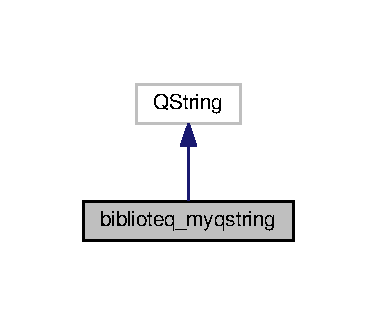
\includegraphics[width=181pt]{classbiblioteq__myqstring__inherit__graph}
\end{center}
\end{figure}


Collaboration diagram for biblioteq\+\_\+myqstring\+:
\nopagebreak
\begin{figure}[H]
\begin{center}
\leavevmode
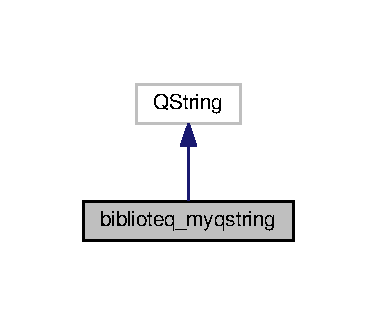
\includegraphics[width=181pt]{classbiblioteq__myqstring__coll__graph}
\end{center}
\end{figure}
\subsection*{Public Member Functions}
\begin{DoxyCompactItemize}
\item 
{\bfseries biblioteq\+\_\+myqstring} (const Q\+String \&str)\hypertarget{classbiblioteq__myqstring_a06f0be4a9667fcd7515f887a8b222b57}{}\label{classbiblioteq__myqstring_a06f0be4a9667fcd7515f887a8b222b57}

\item 
{\bfseries biblioteq\+\_\+myqstring} (const char $\ast$str)\hypertarget{classbiblioteq__myqstring_a7bd6dee31493267f2c572be90b47a9da}{}\label{classbiblioteq__myqstring_a7bd6dee31493267f2c572be90b47a9da}

\item 
Q\+String {\bfseries prep\+Config\+String} (const Q\+String \&str, const bool ignore\+\_\+embedded\+\_\+comments=false)\hypertarget{classbiblioteq__myqstring_a240020e58b9711e8febb705dfc80fb4a}{}\label{classbiblioteq__myqstring_a240020e58b9711e8febb705dfc80fb4a}

\end{DoxyCompactItemize}
\subsection*{Static Public Member Functions}
\begin{DoxyCompactItemize}
\item 
static Q\+String {\bfseries escape} (const Q\+String \&str, const bool caseinsensitive=false)\hypertarget{classbiblioteq__myqstring_ad129d813b76e4393b4ca39c7d210a672}{}\label{classbiblioteq__myqstring_ad129d813b76e4393b4ca39c7d210a672}

\end{DoxyCompactItemize}


The documentation for this class was generated from the following files\+:\begin{DoxyCompactItemize}
\item 
Source/biblioteq\+\_\+myqstring.\+h\item 
Source/biblioteq\+\_\+myqstring.\+cc\end{DoxyCompactItemize}

\hypertarget{classbiblioteq__numeric__table__item}{}\section{biblioteq\+\_\+numeric\+\_\+table\+\_\+item Class Reference}
\label{classbiblioteq__numeric__table__item}\index{biblioteq\+\_\+numeric\+\_\+table\+\_\+item@{biblioteq\+\_\+numeric\+\_\+table\+\_\+item}}


Inheritance diagram for biblioteq\+\_\+numeric\+\_\+table\+\_\+item\+:
\nopagebreak
\begin{figure}[H]
\begin{center}
\leavevmode
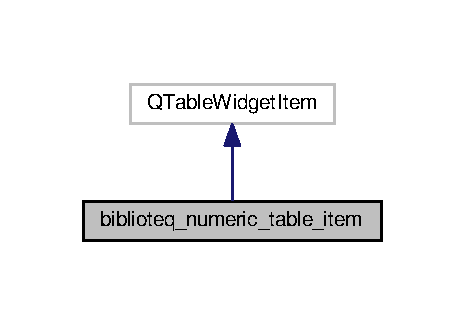
\includegraphics[width=223pt]{classbiblioteq__numeric__table__item__inherit__graph}
\end{center}
\end{figure}


Collaboration diagram for biblioteq\+\_\+numeric\+\_\+table\+\_\+item\+:
\nopagebreak
\begin{figure}[H]
\begin{center}
\leavevmode
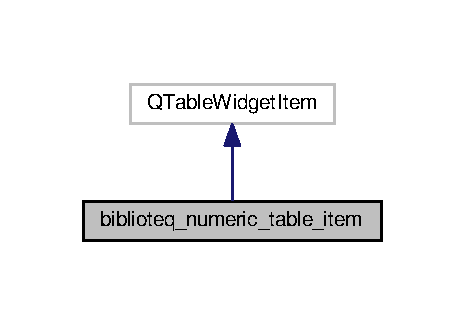
\includegraphics[width=223pt]{classbiblioteq__numeric__table__item__coll__graph}
\end{center}
\end{figure}
\subsection*{Public Member Functions}
\begin{DoxyCompactItemize}
\item 
{\bfseries biblioteq\+\_\+numeric\+\_\+table\+\_\+item} (const double value)\hypertarget{classbiblioteq__numeric__table__item_ac41efd6ef59444e51966d3011ae9a12b}{}\label{classbiblioteq__numeric__table__item_ac41efd6ef59444e51966d3011ae9a12b}

\item 
bool {\bfseries operator$<$} (const Q\+Table\+Widget\+Item \&other) const \hypertarget{classbiblioteq__numeric__table__item_af0e10188fa652bd0e8ebc952a05ae81c}{}\label{classbiblioteq__numeric__table__item_af0e10188fa652bd0e8ebc952a05ae81c}

\end{DoxyCompactItemize}


The documentation for this class was generated from the following files\+:\begin{DoxyCompactItemize}
\item 
Source/biblioteq\+\_\+numeric\+\_\+table\+\_\+item.\+h\item 
Source/biblioteq\+\_\+numeric\+\_\+table\+\_\+item.\+cc\end{DoxyCompactItemize}

\hypertarget{classbiblioteq__otheroptions}{}\section{biblioteq\+\_\+otheroptions Class Reference}
\label{classbiblioteq__otheroptions}\index{biblioteq\+\_\+otheroptions@{biblioteq\+\_\+otheroptions}}


Inheritance diagram for biblioteq\+\_\+otheroptions\+:
\nopagebreak
\begin{figure}[H]
\begin{center}
\leavevmode
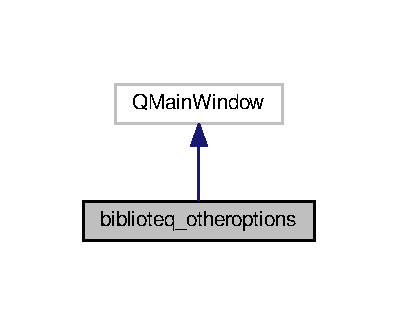
\includegraphics[width=191pt]{classbiblioteq__otheroptions__inherit__graph}
\end{center}
\end{figure}


Collaboration diagram for biblioteq\+\_\+otheroptions\+:
\nopagebreak
\begin{figure}[H]
\begin{center}
\leavevmode
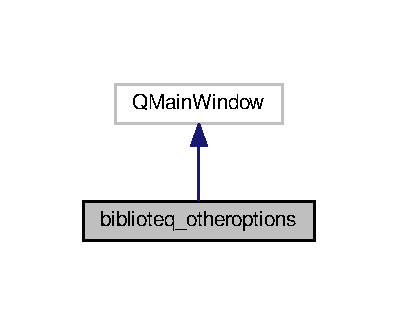
\includegraphics[width=191pt]{classbiblioteq__otheroptions__coll__graph}
\end{center}
\end{figure}
\subsection*{Public Slots}
\begin{DoxyCompactItemize}
\item 
void {\bfseries show\+Normal} (void)\hypertarget{classbiblioteq__otheroptions_a966f360ab5afef4eb7778212ae509384}{}\label{classbiblioteq__otheroptions_a966f360ab5afef4eb7778212ae509384}

\end{DoxyCompactItemize}
\subsection*{Signals}
\begin{DoxyCompactItemize}
\item 
void {\bfseries main\+Window\+Canvas\+Background\+Color\+Changed} (const Q\+Color \&color)\hypertarget{classbiblioteq__otheroptions_ad1fd8fdb291f0ca0221e537d4c5c162c}{}\label{classbiblioteq__otheroptions_ad1fd8fdb291f0ca0221e537d4c5c162c}

\item 
void {\bfseries main\+Window\+Canvas\+Background\+Color\+Preview} (const Q\+Color \&color)\hypertarget{classbiblioteq__otheroptions_aceacb0ae2efa098374082c613d7189b6}{}\label{classbiblioteq__otheroptions_aceacb0ae2efa098374082c613d7189b6}

\item 
void {\bfseries saved} (void)\hypertarget{classbiblioteq__otheroptions_a0bf438e6c64426e26d45d8727c5e1732}{}\label{classbiblioteq__otheroptions_a0bf438e6c64426e26d45d8727c5e1732}

\end{DoxyCompactItemize}
\subsection*{Public Member Functions}
\begin{DoxyCompactItemize}
\item 
Q\+String {\bfseries publication\+Date\+Format} (const Q\+String \&item\+Type) const \hypertarget{classbiblioteq__otheroptions_a1ce7cd5dbef600042498209fe3f77165}{}\label{classbiblioteq__otheroptions_a1ce7cd5dbef600042498209fe3f77165}

\item 
void {\bfseries prepare\+Settings} (void)\hypertarget{classbiblioteq__otheroptions_aa4df15758034cbbc81cae797f6a606b2}{}\label{classbiblioteq__otheroptions_aa4df15758034cbbc81cae797f6a606b2}

\end{DoxyCompactItemize}


The documentation for this class was generated from the following files\+:\begin{DoxyCompactItemize}
\item 
Source/biblioteq\+\_\+otheroptions.\+h\item 
Source/biblioteq\+\_\+otheroptions.\+cc\end{DoxyCompactItemize}

\hypertarget{classbiblioteq__pdfreader}{}\section{biblioteq\+\_\+pdfreader Class Reference}
\label{classbiblioteq__pdfreader}\index{biblioteq\+\_\+pdfreader@{biblioteq\+\_\+pdfreader}}


Inheritance diagram for biblioteq\+\_\+pdfreader\+:
\nopagebreak
\begin{figure}[H]
\begin{center}
\leavevmode
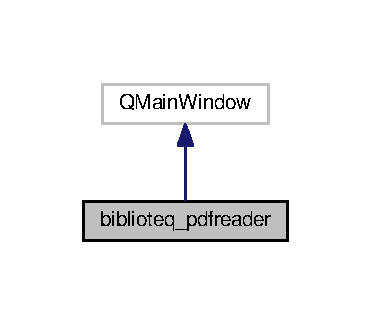
\includegraphics[width=178pt]{classbiblioteq__pdfreader__inherit__graph}
\end{center}
\end{figure}


Collaboration diagram for biblioteq\+\_\+pdfreader\+:
\nopagebreak
\begin{figure}[H]
\begin{center}
\leavevmode
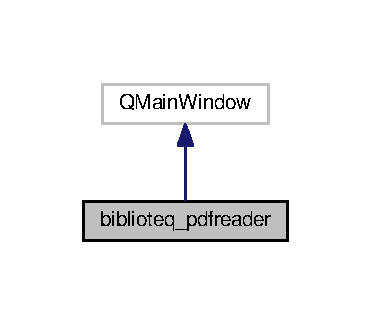
\includegraphics[width=178pt]{classbiblioteq__pdfreader__coll__graph}
\end{center}
\end{figure}
\subsection*{Public Slots}
\begin{DoxyCompactItemize}
\item 
void {\bfseries show\+Normal} (void)\hypertarget{classbiblioteq__pdfreader_ab57800b6bcf4921d5b8acc3d0ab5b6fc}{}\label{classbiblioteq__pdfreader_ab57800b6bcf4921d5b8acc3d0ab5b6fc}

\end{DoxyCompactItemize}
\subsection*{Public Member Functions}
\begin{DoxyCompactItemize}
\item 
{\bfseries biblioteq\+\_\+pdfreader} (Q\+Widget $\ast$parent)\hypertarget{classbiblioteq__pdfreader_a12abb92404fc22a676e65e3215cadb43}{}\label{classbiblioteq__pdfreader_a12abb92404fc22a676e65e3215cadb43}

\item 
void {\bfseries load} (const Q\+Byte\+Array \&data, const Q\+String \&file\+Name)\hypertarget{classbiblioteq__pdfreader_aeb95f9e3b047af92d6106d16166247cd}{}\label{classbiblioteq__pdfreader_aeb95f9e3b047af92d6106d16166247cd}

\item 
void {\bfseries load} (const Q\+String \&file\+Name)\hypertarget{classbiblioteq__pdfreader_ae302c399ad979f274841c79111ad3ffb}{}\label{classbiblioteq__pdfreader_ae302c399ad979f274841c79111ad3ffb}

\end{DoxyCompactItemize}


The documentation for this class was generated from the following files\+:\begin{DoxyCompactItemize}
\item 
Source/biblioteq\+\_\+pdfreader.\+h\item 
Source/biblioteq\+\_\+pdfreader.\+cc\end{DoxyCompactItemize}

\hypertarget{classbiblioteq__photographcollection}{}\section{biblioteq\+\_\+photographcollection Class Reference}
\label{classbiblioteq__photographcollection}\index{biblioteq\+\_\+photographcollection@{biblioteq\+\_\+photographcollection}}


Inheritance diagram for biblioteq\+\_\+photographcollection\+:
\nopagebreak
\begin{figure}[H]
\begin{center}
\leavevmode
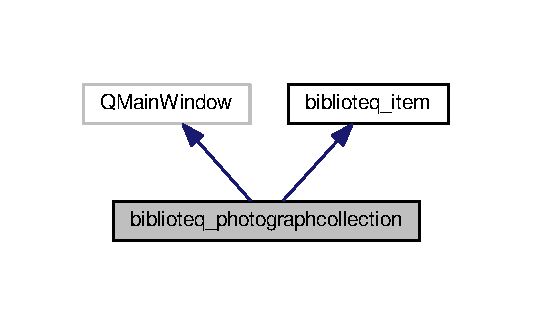
\includegraphics[width=256pt]{classbiblioteq__photographcollection__inherit__graph}
\end{center}
\end{figure}


Collaboration diagram for biblioteq\+\_\+photographcollection\+:
\nopagebreak
\begin{figure}[H]
\begin{center}
\leavevmode
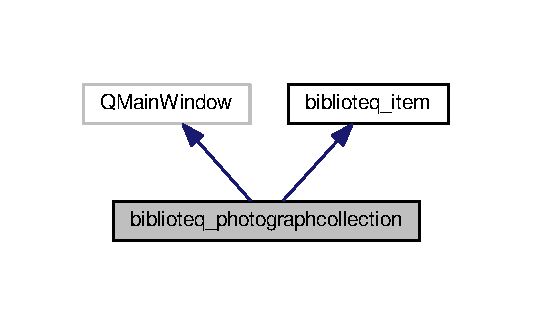
\includegraphics[width=256pt]{classbiblioteq__photographcollection__coll__graph}
\end{center}
\end{figure}
\subsection*{Public Member Functions}
\begin{DoxyCompactItemize}
\item 
{\bfseries biblioteq\+\_\+photographcollection} (Q\+Main\+Window $\ast$parent\+Arg, const Q\+String \&oid\+Arg, const int row\+Arg)\hypertarget{classbiblioteq__photographcollection_ac498eab395a4366771c61796925de6c9}{}\label{classbiblioteq__photographcollection_ac498eab395a4366771c61796925de6c9}

\item 
void {\bfseries duplicate} (const Q\+String \&p\+\_\+oid, const int state)\hypertarget{classbiblioteq__photographcollection_a127c663fb85821551cb1fa0a7a14f63e}{}\label{classbiblioteq__photographcollection_a127c663fb85821551cb1fa0a7a14f63e}

\item 
void {\bfseries insert} (void)\hypertarget{classbiblioteq__photographcollection_aa275b2c143f3f67af3c12ce4964f936d}{}\label{classbiblioteq__photographcollection_aa275b2c143f3f67af3c12ce4964f936d}

\item 
void {\bfseries modify} (const int state, const Q\+String \&behavior=\char`\"{}\char`\"{})\hypertarget{classbiblioteq__photographcollection_a9ba80a269f6b45191a431bfcad60caf5}{}\label{classbiblioteq__photographcollection_a9ba80a269f6b45191a431bfcad60caf5}

\item 
void {\bfseries search} (const Q\+String \&field=\char`\"{}\char`\"{}, const Q\+String \&value=\char`\"{}\char`\"{})\hypertarget{classbiblioteq__photographcollection_a8e8a2e45f3857ce754e4a9a4b054872f}{}\label{classbiblioteq__photographcollection_a8e8a2e45f3857ce754e4a9a4b054872f}

\item 
void {\bfseries set\+Publication\+Date\+Format} (const Q\+String \&date\+Format)\hypertarget{classbiblioteq__photographcollection_af202c0841e35c336c4c2b6bf46e11fab}{}\label{classbiblioteq__photographcollection_af202c0841e35c336c4c2b6bf46e11fab}

\item 
void {\bfseries update\+Window} (const int state)\hypertarget{classbiblioteq__photographcollection_af79d471e654afc1567d818879688bf3f}{}\label{classbiblioteq__photographcollection_af79d471e654afc1567d818879688bf3f}

\end{DoxyCompactItemize}
\subsection*{Static Public Member Functions}
\begin{DoxyCompactItemize}
\item 
static int {\bfseries photographs\+Per\+Page} (void)\hypertarget{classbiblioteq__photographcollection_a9f78f0440562ccbaee24216d49c6e975}{}\label{classbiblioteq__photographcollection_a9f78f0440562ccbaee24216d49c6e975}

\end{DoxyCompactItemize}
\subsection*{Additional Inherited Members}


The documentation for this class was generated from the following files\+:\begin{DoxyCompactItemize}
\item 
Source/biblioteq\+\_\+photographcollection.\+h\item 
Source/biblioteq\+\_\+photographcollection.\+cc\end{DoxyCompactItemize}

\hypertarget{classbiblioteq__sruresults}{}\section{biblioteq\+\_\+sruresults Class Reference}
\label{classbiblioteq__sruresults}\index{biblioteq\+\_\+sruresults@{biblioteq\+\_\+sruresults}}


Inheritance diagram for biblioteq\+\_\+sruresults\+:
\nopagebreak
\begin{figure}[H]
\begin{center}
\leavevmode
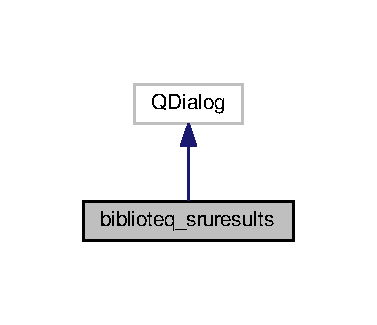
\includegraphics[width=181pt]{classbiblioteq__sruresults__inherit__graph}
\end{center}
\end{figure}


Collaboration diagram for biblioteq\+\_\+sruresults\+:
\nopagebreak
\begin{figure}[H]
\begin{center}
\leavevmode
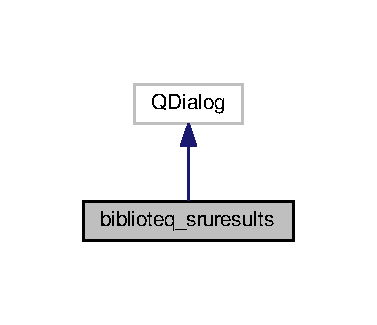
\includegraphics[width=181pt]{classbiblioteq__sruresults__coll__graph}
\end{center}
\end{figure}
\subsection*{Public Member Functions}
\begin{DoxyCompactItemize}
\item 
{\bfseries biblioteq\+\_\+sruresults} (Q\+Widget $\ast$parent, const Q\+List$<$ Q\+Byte\+Array $>$ \&list, \hyperlink{classbiblioteq__magazine}{biblioteq\+\_\+magazine} $\ast$magazine\+\_\+arg, const Q\+Font \&font)\hypertarget{classbiblioteq__sruresults_a6d5677e14e69a168c05679f9db7ecf7c}{}\label{classbiblioteq__sruresults_a6d5677e14e69a168c05679f9db7ecf7c}

\end{DoxyCompactItemize}


The documentation for this class was generated from the following files\+:\begin{DoxyCompactItemize}
\item 
Source/biblioteq\+\_\+sru\+Results.\+h\item 
Source/biblioteq\+\_\+sru\+Results.\+cc\end{DoxyCompactItemize}

\hypertarget{classbiblioteq__videogame}{}\section{biblioteq\+\_\+videogame Class Reference}
\label{classbiblioteq__videogame}\index{biblioteq\+\_\+videogame@{biblioteq\+\_\+videogame}}


Inheritance diagram for biblioteq\+\_\+videogame\+:
\nopagebreak
\begin{figure}[H]
\begin{center}
\leavevmode
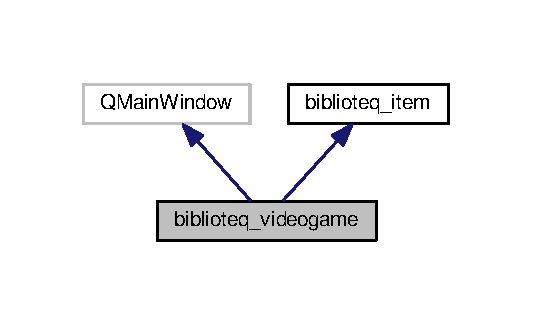
\includegraphics[width=256pt]{classbiblioteq__videogame__inherit__graph}
\end{center}
\end{figure}


Collaboration diagram for biblioteq\+\_\+videogame\+:
\nopagebreak
\begin{figure}[H]
\begin{center}
\leavevmode
\includegraphics[width=256pt]{classbiblioteq__videogame__coll__graph}
\end{center}
\end{figure}
\subsection*{Public Member Functions}
\begin{DoxyCompactItemize}
\item 
{\bfseries biblioteq\+\_\+videogame} (Q\+Main\+Window $\ast$pareng\+Arg, const Q\+String \&oid\+Arg, const int row\+Arg)\hypertarget{classbiblioteq__videogame_a089bc36f7535fee9fa4edd329ac3d5f7}{}\label{classbiblioteq__videogame_a089bc36f7535fee9fa4edd329ac3d5f7}

\item 
void {\bfseries duplicate} (const Q\+String \&p\+\_\+oid, const int state)\hypertarget{classbiblioteq__videogame_abd19c8c36646158bdda33075236e4922}{}\label{classbiblioteq__videogame_abd19c8c36646158bdda33075236e4922}

\item 
void {\bfseries insert} (void)\hypertarget{classbiblioteq__videogame_ad9456c707dbfb382d83b26890e70fd84}{}\label{classbiblioteq__videogame_ad9456c707dbfb382d83b26890e70fd84}

\item 
void {\bfseries modify} (const int state)\hypertarget{classbiblioteq__videogame_acc0e4822674716ef5b4eb838d10bcaed}{}\label{classbiblioteq__videogame_acc0e4822674716ef5b4eb838d10bcaed}

\item 
void {\bfseries search} (const Q\+String \&field=\char`\"{}\char`\"{}, const Q\+String \&value=\char`\"{}\char`\"{})\hypertarget{classbiblioteq__videogame_a42dbc4359bd2d8563f18f9ccbc37b5d9}{}\label{classbiblioteq__videogame_a42dbc4359bd2d8563f18f9ccbc37b5d9}

\item 
void {\bfseries set\+Publication\+Date\+Format} (const Q\+String \&date\+Format)\hypertarget{classbiblioteq__videogame_a3bb1fe56621b3c0eddc147336f0bf000}{}\label{classbiblioteq__videogame_a3bb1fe56621b3c0eddc147336f0bf000}

\item 
void {\bfseries update\+Window} (const int state)\hypertarget{classbiblioteq__videogame_a6a062a4e4eec4fd507f32d210a612034}{}\label{classbiblioteq__videogame_a6a062a4e4eec4fd507f32d210a612034}

\end{DoxyCompactItemize}
\subsection*{Additional Inherited Members}


The documentation for this class was generated from the following files\+:\begin{DoxyCompactItemize}
\item 
Source/biblioteq\+\_\+videogame.\+h\item 
Source/biblioteq\+\_\+videogame.\+cc\end{DoxyCompactItemize}

\hypertarget{classbiblioteq__z3950results}{}\section{biblioteq\+\_\+z3950results Class Reference}
\label{classbiblioteq__z3950results}\index{biblioteq\+\_\+z3950results@{biblioteq\+\_\+z3950results}}


Inheritance diagram for biblioteq\+\_\+z3950results\+:
\nopagebreak
\begin{figure}[H]
\begin{center}
\leavevmode
\includegraphics[width=193pt]{classbiblioteq__z3950results__inherit__graph}
\end{center}
\end{figure}


Collaboration diagram for biblioteq\+\_\+z3950results\+:
\nopagebreak
\begin{figure}[H]
\begin{center}
\leavevmode
\includegraphics[width=193pt]{classbiblioteq__z3950results__coll__graph}
\end{center}
\end{figure}
\subsection*{Public Member Functions}
\begin{DoxyCompactItemize}
\item 
{\bfseries biblioteq\+\_\+z3950results} (Q\+Widget $\ast$parent, Q\+String\+List \&list, \hyperlink{classbiblioteq__magazine}{biblioteq\+\_\+magazine} $\ast$magazine\+\_\+arg, const Q\+Font \&font, const Q\+String \&record\+Syntax)\hypertarget{classbiblioteq__z3950results_a74c0325525d70d87c41a43de748b8e23}{}\label{classbiblioteq__z3950results_a74c0325525d70d87c41a43de748b8e23}

\end{DoxyCompactItemize}


The documentation for this class was generated from the following files\+:\begin{DoxyCompactItemize}
\item 
Source/biblioteq\+\_\+z3950results.\+h\item 
Source/biblioteq\+\_\+z3950results.\+cc\end{DoxyCompactItemize}

\hypertarget{classCocoaInitializer}{}\section{Cocoa\+Initializer Class Reference}
\label{classCocoaInitializer}\index{Cocoa\+Initializer@{Cocoa\+Initializer}}
\subsection*{Classes}
\begin{DoxyCompactItemize}
\item 
class \hyperlink{classCocoaInitializer_1_1Private}{Private}
\end{DoxyCompactItemize}


The documentation for this class was generated from the following files\+:\begin{DoxyCompactItemize}
\item 
Source/Cocoa\+Initializer.\+h\item 
Source/Cocoa\+Initializer.\+mm\end{DoxyCompactItemize}

\hypertarget{classCocoaInitializer_1_1Private}{}\section{Cocoa\+Initializer\+:\+:Private Class Reference}
\label{classCocoaInitializer_1_1Private}\index{Cocoa\+Initializer\+::\+Private@{Cocoa\+Initializer\+::\+Private}}
\subsection*{Public Attributes}
\begin{DoxyCompactItemize}
\item 
N\+S\+Autorelease\+Pool $\ast$ {\bfseries auto\+Release\+Pool\+\_\+}\hypertarget{classCocoaInitializer_1_1Private_a8242bed2abdec29f1cf8745d6d9c0e7d}{}\label{classCocoaInitializer_1_1Private_a8242bed2abdec29f1cf8745d6d9c0e7d}

\end{DoxyCompactItemize}


The documentation for this class was generated from the following file\+:\begin{DoxyCompactItemize}
\item 
Source/Cocoa\+Initializer.\+mm\end{DoxyCompactItemize}

\hypertarget{classuserinfo__diag__class}{}\section{userinfo\+\_\+diag\+\_\+class Class Reference}
\label{classuserinfo__diag__class}\index{userinfo\+\_\+diag\+\_\+class@{userinfo\+\_\+diag\+\_\+class}}


Inheritance diagram for userinfo\+\_\+diag\+\_\+class\+:
\nopagebreak
\begin{figure}[H]
\begin{center}
\leavevmode
\includegraphics[width=183pt]{classuserinfo__diag__class__inherit__graph}
\end{center}
\end{figure}


Collaboration diagram for userinfo\+\_\+diag\+\_\+class\+:
\nopagebreak
\begin{figure}[H]
\begin{center}
\leavevmode
\includegraphics[width=183pt]{classuserinfo__diag__class__coll__graph}
\end{center}
\end{figure}
\subsection*{Public Member Functions}
\begin{DoxyCompactItemize}
\item 
{\bfseries userinfo\+\_\+diag\+\_\+class} (Q\+Main\+Window $\ast$parent)\hypertarget{classuserinfo__diag__class_a068606f4ea35d4818b2f843a7ff16365}{}\label{classuserinfo__diag__class_a068606f4ea35d4818b2f843a7ff16365}

\item 
bool {\bfseries have\+Member\+Changes} (Q\+String \&str)\hypertarget{classuserinfo__diag__class_a76504f0e16c84b63f2f06560f47b42d6}{}\label{classuserinfo__diag__class_a76504f0e16c84b63f2f06560f47b42d6}

\end{DoxyCompactItemize}
\subsection*{Public Attributes}
\begin{DoxyCompactItemize}
\item 
Q\+Hash$<$ Q\+String, Q\+String $>$ {\bfseries m\+\_\+member\+Properties}\hypertarget{classuserinfo__diag__class_adf5b60bdacd18cd87fc70a956a63454b}{}\label{classuserinfo__diag__class_adf5b60bdacd18cd87fc70a956a63454b}

\item 
Ui\+\_\+\+User\+Info {\bfseries m\+\_\+userinfo}\hypertarget{classuserinfo__diag__class_a341e3da03b4472e1603b417323876995}{}\label{classuserinfo__diag__class_a341e3da03b4472e1603b417323876995}

\end{DoxyCompactItemize}


The documentation for this class was generated from the following file\+:\begin{DoxyCompactItemize}
\item 
Source/biblioteq.\+h\end{DoxyCompactItemize}

%--- End generated contents ---

% Index
\backmatter
\newpage
\phantomsection
\clearemptydoublepage
\addcontentsline{toc}{chapter}{Index}
\printindex

\end{document}
